%% The first command in your LaTeX source must be the \documentclass command.
\documentclass[manuscript,screen,review]{acmart}

%% NOTE that a single column version is required for 
%% submission and peer review. This can be done by changing
%% the \doucmentclass[...]{acmart} in this template to 
%% \documentclass[manuscript,screen,review]{acmart}
%% 
%% To ensure 100% compatibility, please check the white list of
%% approved LaTeX packages to be used with the Master Article Template at
%% https://www.acm.org/publications/taps/whitelist-of-latex-packages 
%% before creating your document. The white list page provides 
%% information on how to submit additional LaTeX packages for 
%% review and adoption.
%% Fonts used in the template cannot be substituted; margin 
%% adjustments are not allowed.
%%
%% \BibTeX command to typeset BibTeX logo in the docs
\AtBeginDocument{%
  \providecommand\BibTeX{{%
    \normalfont B\kern-0.5em{\scshape i\kern-0.25em b}\kern-0.8em\TeX}}}

%% Rights management information.  This information is sent to you
%% when you complete the rights form.  These commands have SAMPLE
%% values in them; it is your responsibility as an author to replace
%% the commands and values with those provided to you when you
%% complete the rights form.
\setcopyright{acmcopyright}
\copyrightyear{2021}
\acmYear{2021}
\acmDOI{10.1145/1122445.1122456}


%%
%% These commands are for a JOURNAL article.
% \acmJournal{POMACS}
% \acmVolume{37}
% \acmNumber{4}
% \acmArticle{111}
% \acmMonth{8}

% *** MACRO FOR MARKING TODO's ***
\usepackage{xcolor}
\newcommand{\todo}[1]{\textcolor{red}{\textbf{\underline{TODO:}} #1}}
\newcommand{\patrick}[1]{\textcolor{blue}{\textbf{\underline{PM:}} #1}}
\newcommand{\ttj}[1]{\textcolor{red}{\textbf{\underline{TTJ:}} #1}}
\newcommand{\diego}[1]{\textcolor{purple}{\textbf{\underline{DM:}} #1}}

% \renewcommand{\todo}[1]{}
% \renewcommand{\patrick}[1]{}
% \renewcommand{\ttj}[1]{}

% \usepackage{todonotes}

\usepackage{color, colortbl}
\definecolor{Gray}{gray}{0.9}
\usepackage{algorithmic}
\usepackage[ruled]{algorithm2e}
\usepackage{graphicx}
\usepackage{multirow}
\usepackage[bottom]{footmisc}



%%
%% The majority of ACM publications use numbered citations and
%% references.  The command \citestyle{authoryear} switches to the
%% "author year" style.
%%
%% If you are preparing content for an event
%% sponsored by ACM SIGGRAPH, you must use the "author year" style of
%% citations and references.
%% Uncommenting
%% the next command will enable that style.
%%\citestyle{acmauthoryear}

%%
%% end of the preamble, start of the body of the document source.
\begin{document}

%%
%% The "title" command has an optional parameter,
%% allowing the author to define a "short title" to be used in page headers.
\title{Online Safety Assurance for Machine learning Controllers with Real-Time Reachability}

%%
%% The "author" command and its associated commands are used to define
%% the authors and their affiliations.
%% Of note is the shared affiliation of the first two authors, and the
%% "authornote" and "authornotemark" commands
%% used to denote shared contribution to the research.

\author{Patrick Musau}
\affiliation{%
  \institution{Vanderbilt University}
  \city{Nashville}
  \state{TN}
  \country{USA}
  \postcode{37215}
}


\author{Nathaniel Hamilton}
\affiliation{%
  \institution{Vanderbilt University}
  \city{Nashville}
  \state{TN}
  \country{USA}
  \postcode{37215}
}

\author{Diego Manzanas Lopez}
\affiliation{%
  \institution{Vanderbilt University}
  \city{Nashville}
  \state{TN}
  \country{USA}
  \postcode{37215}
}

\author{Preston Robinette}
\affiliation{%
  \institution{Vanderbilt University}
  \city{Nashville}
  \state{TN}
  \country{USA}
  \postcode{37215}
}

\author{Taylor T. Johnson}
\affiliation{%
  \institution{Vanderbilt University}
  \city{Nashville}
  \state{TN}
  \country{USA}
  \postcode{37215}
}


%%
%% By default, the full list of authors will be used in the page
%% headers. Often, this list is too long, and will overlap
%% other information printed in the page headers. This command allows
%% the author to define a more concise list
%% of authors' names for this purpose.
\renewcommand{\shortauthors}{Musau et al.}

%%
%% The abstract is a short summary of the work to be presented in the
%% article.
\begin{abstract}
  Recent advances in Artificial Intelligence research has led to the emergence of machine learning models deployed within safety critical systems, where they are often used for sensing, actuation, and control. Despite the prolific advances that have been enabled by machine learning methods, such systems are notoriously difficult to assure. The challenge here is that some models, such as neural networks, are ``black box'' in nature, making verification and validation difficult and sometimes infeasible. One approach to provide assurance of systems with unverified components is the simplex architecture, where an unverified component is wrapped with a safety controller and a switching logic designed to prevent dangerous behavior. In this manuscript, we evaluate such an architecture for the safety assurance of a one-tenth scale autonomous car through the use of a real-time reachability algorithm to (a) provide provable guarantees of safety and (b) detect potentially unsafe scenarios. We demonstrate the efficacy of the proposed runtime verification approach through experiments conducted both in simulation and on an embedded hardware platform. Furthermore, we present a characterization of the execution times on both platforms, validating the real-time aspects of our approach.
\end{abstract}

%%
%% The code below is generated by the tool at http://dl.acm.org/ccs.cfm.
%% Please copy and paste the code instead of the example below.
%%
% \begin{CCSXML}
% <ccs2012>
%  <concept>
%   <concept_id>10010520.10010553.10010562</concept_id>
%   <concept_desc>Computer systems organization~Embedded systems</concept_desc>
%   <concept_significance>500</concept_significance>
%  </concept>
%  <concept>
%   <concept_id>10010520.10010575.10010755</concept_id>
%   <concept_desc>Computer systems organization~Redundancy</concept_desc>
%   <concept_significance>300</concept_significance>
%  </concept>
%  <concept>
%   <concept_id>10010520.10010553.10010554</concept_id>
%   <concept_desc>Computer systems organization~Robotics</concept_desc>
%   <concept_significance>100</concept_significance>
%  </concept>
%  <concept>
%   <concept_id>10003033.10003083.10003095</concept_id>
%   <concept_desc>Networks~Network reliability</concept_desc>
%   <concept_significance>100</concept_significance>
%  </concept>
% </ccs2012>
% \end{CCSXML}

% \ccsdesc[500]{Computer systems organization~Embedded systems}
% \ccsdesc[300]{Computer systems organization~Redundancy}
% \ccsdesc{Computer systems organization~Robotics}
% \ccsdesc[100]{Networks~Network reliability}


% \keywords{datasets, neural networks, gaze detection, text tagging}



\maketitle

\section{Introduction}
%\todo{Need to change this so that it doesn't include anything from the IROS Paper. Do this last, as this highly depends on the results of other efforts. Part of the story of this paper is that training agents in simulation and then deploying them on real-hardware is a challenging problem. In many cases, the agents do not perform as well as expected. With a set of four controllers that we deploy on real-hardware this can be effectively communicated as an overall story.}


The vision of a "driverless" future has riveted many technology enthusiasts, researchers, and corporations for decades \cite{Badue2019}. The prevailing sensitivity is that there are relatively few technologies that holds as much promise as autonomous vehicles (AVs) in bringing about safe, accessible, and convenient transportation. Particulary, when the status-quo is considered, far too many individuals still lose their lives to traffic fatalities each year \cite{Rasouli2020}. As Koopman et al. write, "The question is not whether or not autonomous vehicles will be perfect. The question is when [will] we be able to deploy a fleet of fully autonomous driving systems that are actually safe enough to leave the human completely out of the driving loop" \cite{Koopman2017}.
\raggedbottom

The two fundamental challenges that are widely regarded as limiting the arrival and widespread adoption of AVs are safety and reliability \cite{Majumdar2017}. Reasoning about safety requires an understanding of the joint dynamics of computers, networks, and physical dynamics, in uncertain and variable environments \cite{Yurtsever2019}. Consequently, it is a notoriously difficult problem. Additionally, to handle the complexities of their environments, many AVs make use to machine learning (ML) components to make sense of information observed from an ever-evolving configuration of on-board sensors \cite{Yurtsever2019}. Despite the impressive capabilities of these components, there are reservations about using them within safety-critical settings due to their largely opaque nature. This prevents meaningful statements about their behavior from being made. Utilizing a ``black-box'' model within a system that is safety-critical constitutes the highest form of technical debt \cite{Sculley2015} and, as a result, the last several years have witnessed a significant increase in the development of methods that seek to reason about the safety and robustness of machine learning methods \cite{xiang20118survey}.






%For decades, many technology enthusiasts, researchers, and corporations have had visions of deploying autonomous vehicles on the road~\cite{boudette_2019, Badue2019}. These visions were further emboldened by the success of challenges organized by the Defense Advanced Research Projects Agency (DARPA)~\cite{DARPA_Challenge,driverless_challenges}. The challenges demonstrated the proliferation of autonomous vehicle technology as a vision that could be achieved and spurred the growth of research centers and hundreds of autonomous vehicle companies such as Alphabet's WAYMO, Uber ATG, Argo AI, Aptiv, ZOOX, General Motors' Cruise, Tesla, Aurora, and Intel Corporation's Mobileye \cite{Companies}. While initial projections estimated that autonomous vehicles would be roaming our streets by 2020, today many companies have concluded that the development of robust and safe autonomous vehicles is going to be harder, slower, and more costly than they had originally estimated \cite{driverless_challenges}.

%Among the numerous challenges within this sector, safety is a notoriously difficult problem, and solutions that are both rigorous and practical have yet to be realized \cite{Allen2014}. Autonomous vehicles operate in uncertain, and often unknown environments. Additionally, their perception of this dynamic environment is limited to an ever evolving configuration of on-board sensors \cite{Yurtsever2019}. Within this context, the auspicious results of machine learning methods such as reinforcement learning and deep learning have generated a considerable amount of excitement due to their impressive capabilities in dealing with complex data. However, there are reservations about using them within safety-critical settings due to the difficulty of interpreting the inner workings of these models, which prevents any meaningful statements about their behavior from being made. 

%Typically, in simplex architectures, the switching logic is primarily designed either from a control theoretic perspective through the solution of linear matrix inequalities (LMI) \cite{SetoCaseStudy2000}, or using a formal analysis hybrid-systems reachability technique \cite{Bak2009Simplex}.

Unfortunately, while numerous works have been proposed in the past few years for the formal analysis of machine learning methods, designing solutions that are both practical and rigorous is extremely challenging. Particularly, in the context of ML models such as neural networks that may be characterized by millions or even billions of parameters \cite{BallesterGoogLeNet,SimonyanVeryDeep}. One approach that has enabled the assurance of systems with unverified components is the \textit{simplex architecture}. In this framework, an unverified component is wrapped with a safety controller and switching logic designed to transfer control to the safety controller in certain situations \cite{Bak2014}. The key challenge in this regime is to design a switching logic that allows the dynamic capabilities of the unverified, complex controller to be exploited without compromising safety. In this manuscript, we extend a real-time reachability algorithm \cite{Bak2014,Johnson2016} to design a simplex architecture for a $1/10$ scale autonomous racing car called the F1/10 platform. \diego{I see the point of this paragraph, but it could be confusing. Simplex is an architecture used to switch controllers, it is not a formal analysis of NNs. I will add maybe one more sentence clarifying that there are other ways of dealing with nn controllers such as simplex, or other runtime monitoring/assurance methods that reason about the system while operating, instead of reasoning about the controller at design/offline time. You mention that this work is runtime assurance in the next paragraph, but if I did not know what you are trying to do, I'd be confused}

In order to put our work into context, this work falls within the \textit{run-time verification} or \textit{run-time assurance} realm. Our aim is to construct an architecture that allows us to ensure that an autonomous vehicle, controlled using machine learning strategies, never enters unsafe states as it navigates within an environment. Specifically, the set of control strategies presented herein were synthesized using reinforcement learning and imitation learning, which have generated a considerable amount of excitement in recent years \diego{Maybe add citation for that "excitement claim?}. Our approach abstracts away the need to analyze the underlying nature of the controller and instead observes the influence of control actions on the systems behavior at runtime. This makes it particularly applicable to machine learning systems. 
%\todo{I can replace this figure of the F1Tenth with another one. This one has already been submitted to another conference.}
%\begin{figure}%[htp!]
%  \centering
%    % \hspace*{-8mm}  
%    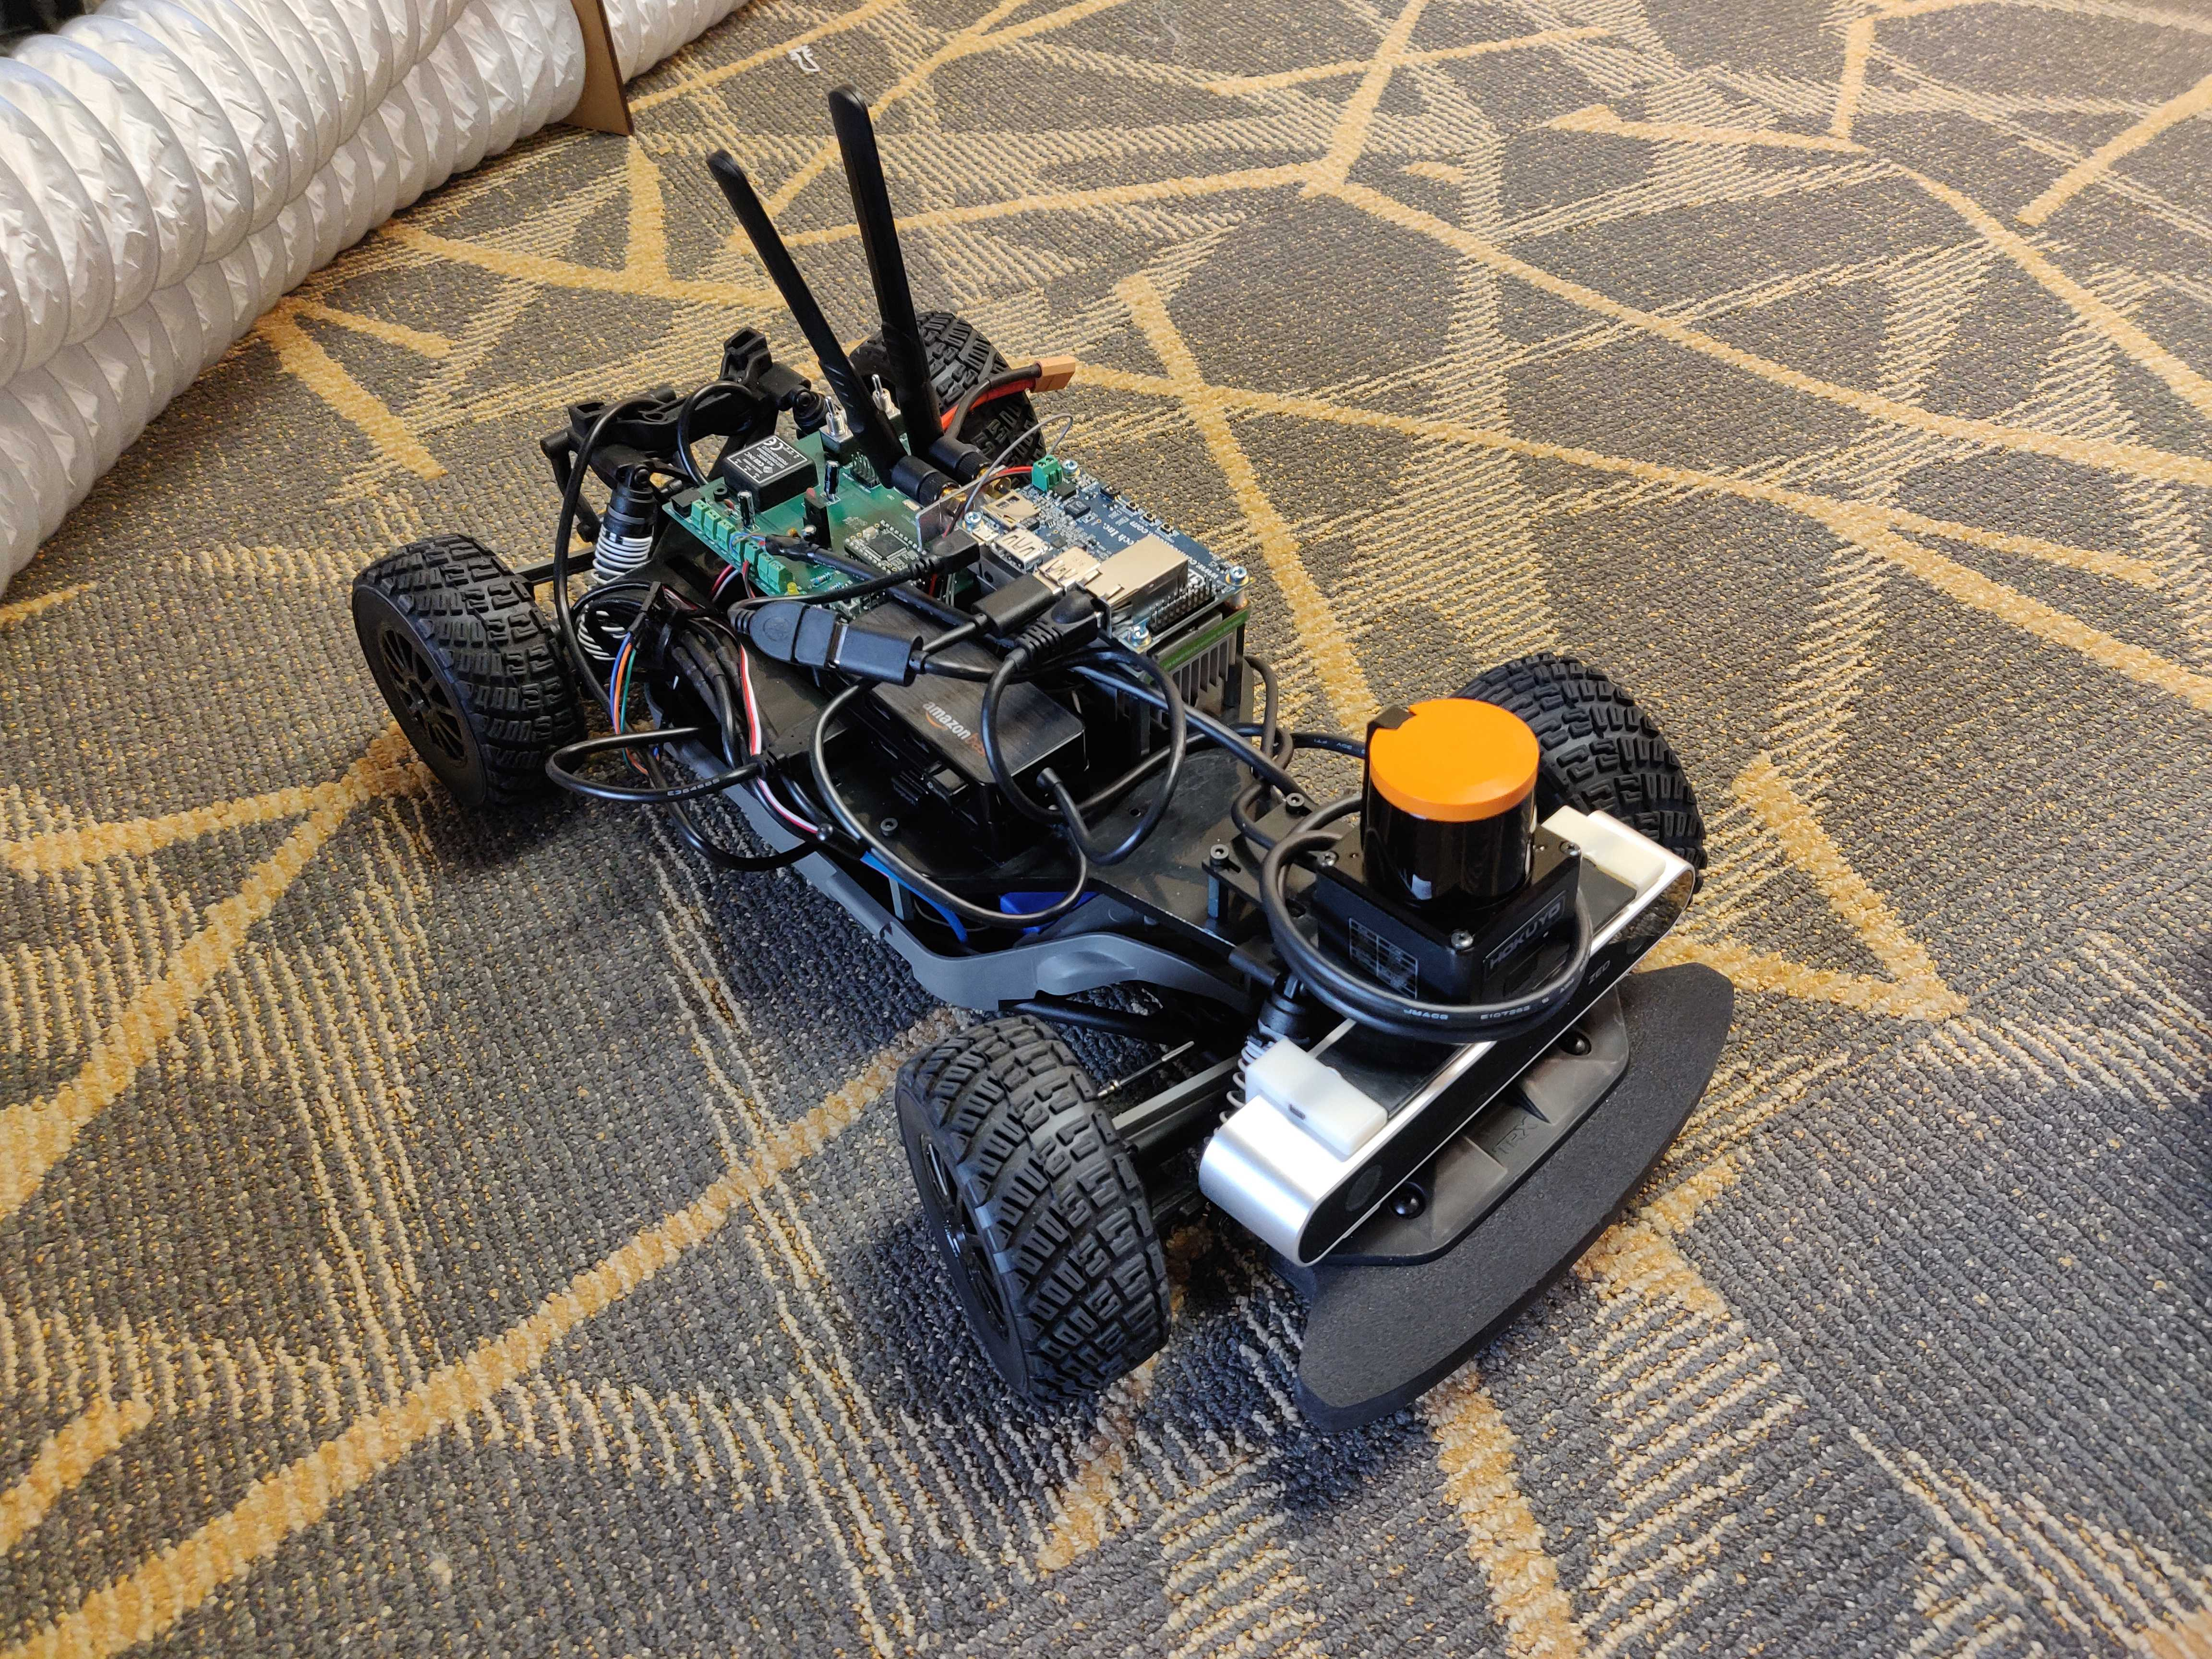
\includegraphics[width=0.5\linewidth]{f1tenth.jpg}
%   \caption{Visualization of our experimental F1/10 hardware platform. This platform is a one-tenth scale RC car that has been altered to entertain autonomous control inputs as well as support a sensor and compute architecture for autonomous decision making. \cite{okelly2020}. }
%  \label{fig:f1tenth_hardware}
%\end{figure}

To perform the verification, we first identify a dynamical model of the car and assume that the car operates within an \textit{a priori} known environment. Next, we synthesize controllers, using data collected from a series of experiments with the F1/10 vehicle, as well as through the execution of a series of reinforcement learning training campaigns. Using the obtained controllers, we aim to verify that the car does not crash with static obstacles within its environment as well as the environment boundaries. To do this, we extend a real-time reachability algorithm proposed by Bak et al. \cite{Bak2014,Johnson2016} to compute the set of reachable states for a finite time-horizon and check for potential collisions. This safety checking forms the basis of the switching scheme in our simplex architecture, and we evaluate the merits of this approach both in simulation and on the F1/10 hardware platform using a variety of controllers, number of obstacles, and run-time configurations.

In summary, the contributions of this manuscript are: 
\begin{itemize}
    \item We extend a previous simplex control architecture that makes use of a real-time reachability algorithm based on mixed face-lifting to an autonomous race car both in simulation and on an embedded platform.
    \item The presentation of a regime that abstracts away the need to analyze opaque machine learning models, and instead observes the influence of their decisions on the system during operation.
    %\item We train two learning-enabled, or ``black-box'', controllers.
    \item We demonstrate success using the simplex architecture to safely navigate through obstacles, with which the trained controllers had no prior experience.
    \item An evaluation of the safety of machine learning components transferred to real-world hardware without additional training.
\end{itemize}

\diego{Very good description of contributions!!}
\section{Background: The Simplex Architecture and Real-Time Reachability}
% \todo{introduce topic. Poor form to start a section with a subsection}

\subsection{Simplex Architecture}

%As modern autonomous systems grow in complexity, so do the challenges in assessing their reliability and correctness \cite{Bak2009Simplex}. Moreover, any arguments about the reliability and safety of the system rely on assertions about the individual components that make it up \cite{Bak2014}. However, in recent years, with the growth of increasingly autonomous systems \cite{Jha2020}, individual components may be designed using machine learning methods, such as neural networks, that are opaque to traditional formal analysis. Despite the recent years' surge in the development of formal analysis techniques for these types of models \cite{Liu2019,xiang20118survey}, most techniques are incapable of dealing with the scale of models deployed in state-of-the-art systems.

One paradigm for dealing with untrustworthy components is the \emph{simplex architecture} \cite{RiveraAnArchitectural1996}. In the simplex architecture, the unverified component, or \emph{complex controller}, is wrapped with a \emph{safety controller} and a switching logic used to ensure safety~\cite{Bak2014}. A useful analogy for this architecture is a driving instructor's car with two steering wheels and two sets of brakes. As long as the instructor is capable of intervening in dangerous situations, the capricious student is allowed to drive. Typically, the complex controller has better performance with respect to the design metrics, whereas the safety controller is designed with simplicity and verifiability in mind. Thus, by using this architecture, one can utilize the complex controller while still maintaining the formal guarantees of the safety controller. The key challenge when designing a system with the simplex architecture is properly designing the switching logic \cite{Johnson2016}. One must be able to clearly delineate safe states from unsafe states. 

Typically, in simplex architectures, the switching logic is primarily designed either from a control theoretic perspective through the solution of linear matrix inequalities (LMI) \cite{SetoCaseStudy2000}, or using a formal analysis hybrid-systems reachability technique \cite{Bak2009Simplex}. In this manuscript, our simplex design necessitates computing the set of reachable states online through the use of a real-time reachability algorithm for short time horizons.

\subsection{Real-Time Reachability}

Reachability algorithms have traditionally been executed offline and are typically computationally intensive endeavors \cite{Chen2013,AlthoffCORA2015,manzanas2019arch_ainncs}. However, in \cite{Bak2014,Johnson2016}, Bak et al., and Johnson et al. presented a reachability algorithm, based on the influential mixed face-lifting algorithm \cite{dang2000}, capable of running in real-time on embedded processors. The algorithm is implemented as a standalone C-package that does not rely on sophisticated (non-portable) libraries, recursion, or dynamic data structures and is amenable to the anytime computation model in the real-time scheduling literature \cite{Liu1991}. In this regime, each task produces a partial result that is improved upon as more computation time is added \cite{Johnson2016}. 

%todo{Define Reachability Similar to How I defined it for the IROS Paper}
%Before briefly outlining the algorithm, let us define \emph{reach-time} as the time we spend computing the reachable set, and \emph{runtime}, as the duration of (wall) time the method is allowed to run. With that, the real-time reachability algorithm works as follows. 

The controllers used in our experiments are designed to sample sensor data and compute control actions at fixed time intervals as typically done in the control community \cite{Dai2020}. During each control period, we take the corresponding control action and compute the reachable set of states into the future as defined by the current state and a specified finite-time horizon. An example of this computation is shown in Figure~\ref{fig:reachset}. We assume a fixed control action throughout the reachable set computation. Based on the obtained reachable set, we determine if the system will collide with objects in its environment and, if necessary, switch to a safety controller optimized for obstacle avoidance. If the system falls back to using a safety controller, we only allow a switch back to the complex controller if the complex controller has demonstrated safe behavior for a fixed number of control periods. This is to prevent arbitrary switching and to incorporate a sense of hysteresis into our control strategy. Additionally, by not switching back until consistently safe behavior has been demonstrated, we enforce a notion of dwell time, which reduces instabilities caused by switching too frequently. Our approach has successfully been deployed to ensure safety both in simulation and on the F1/10 hardware platform.

\begin{figure}[htpb]%[!htb]
  \centering
    % \hspace*{-8mm}  
    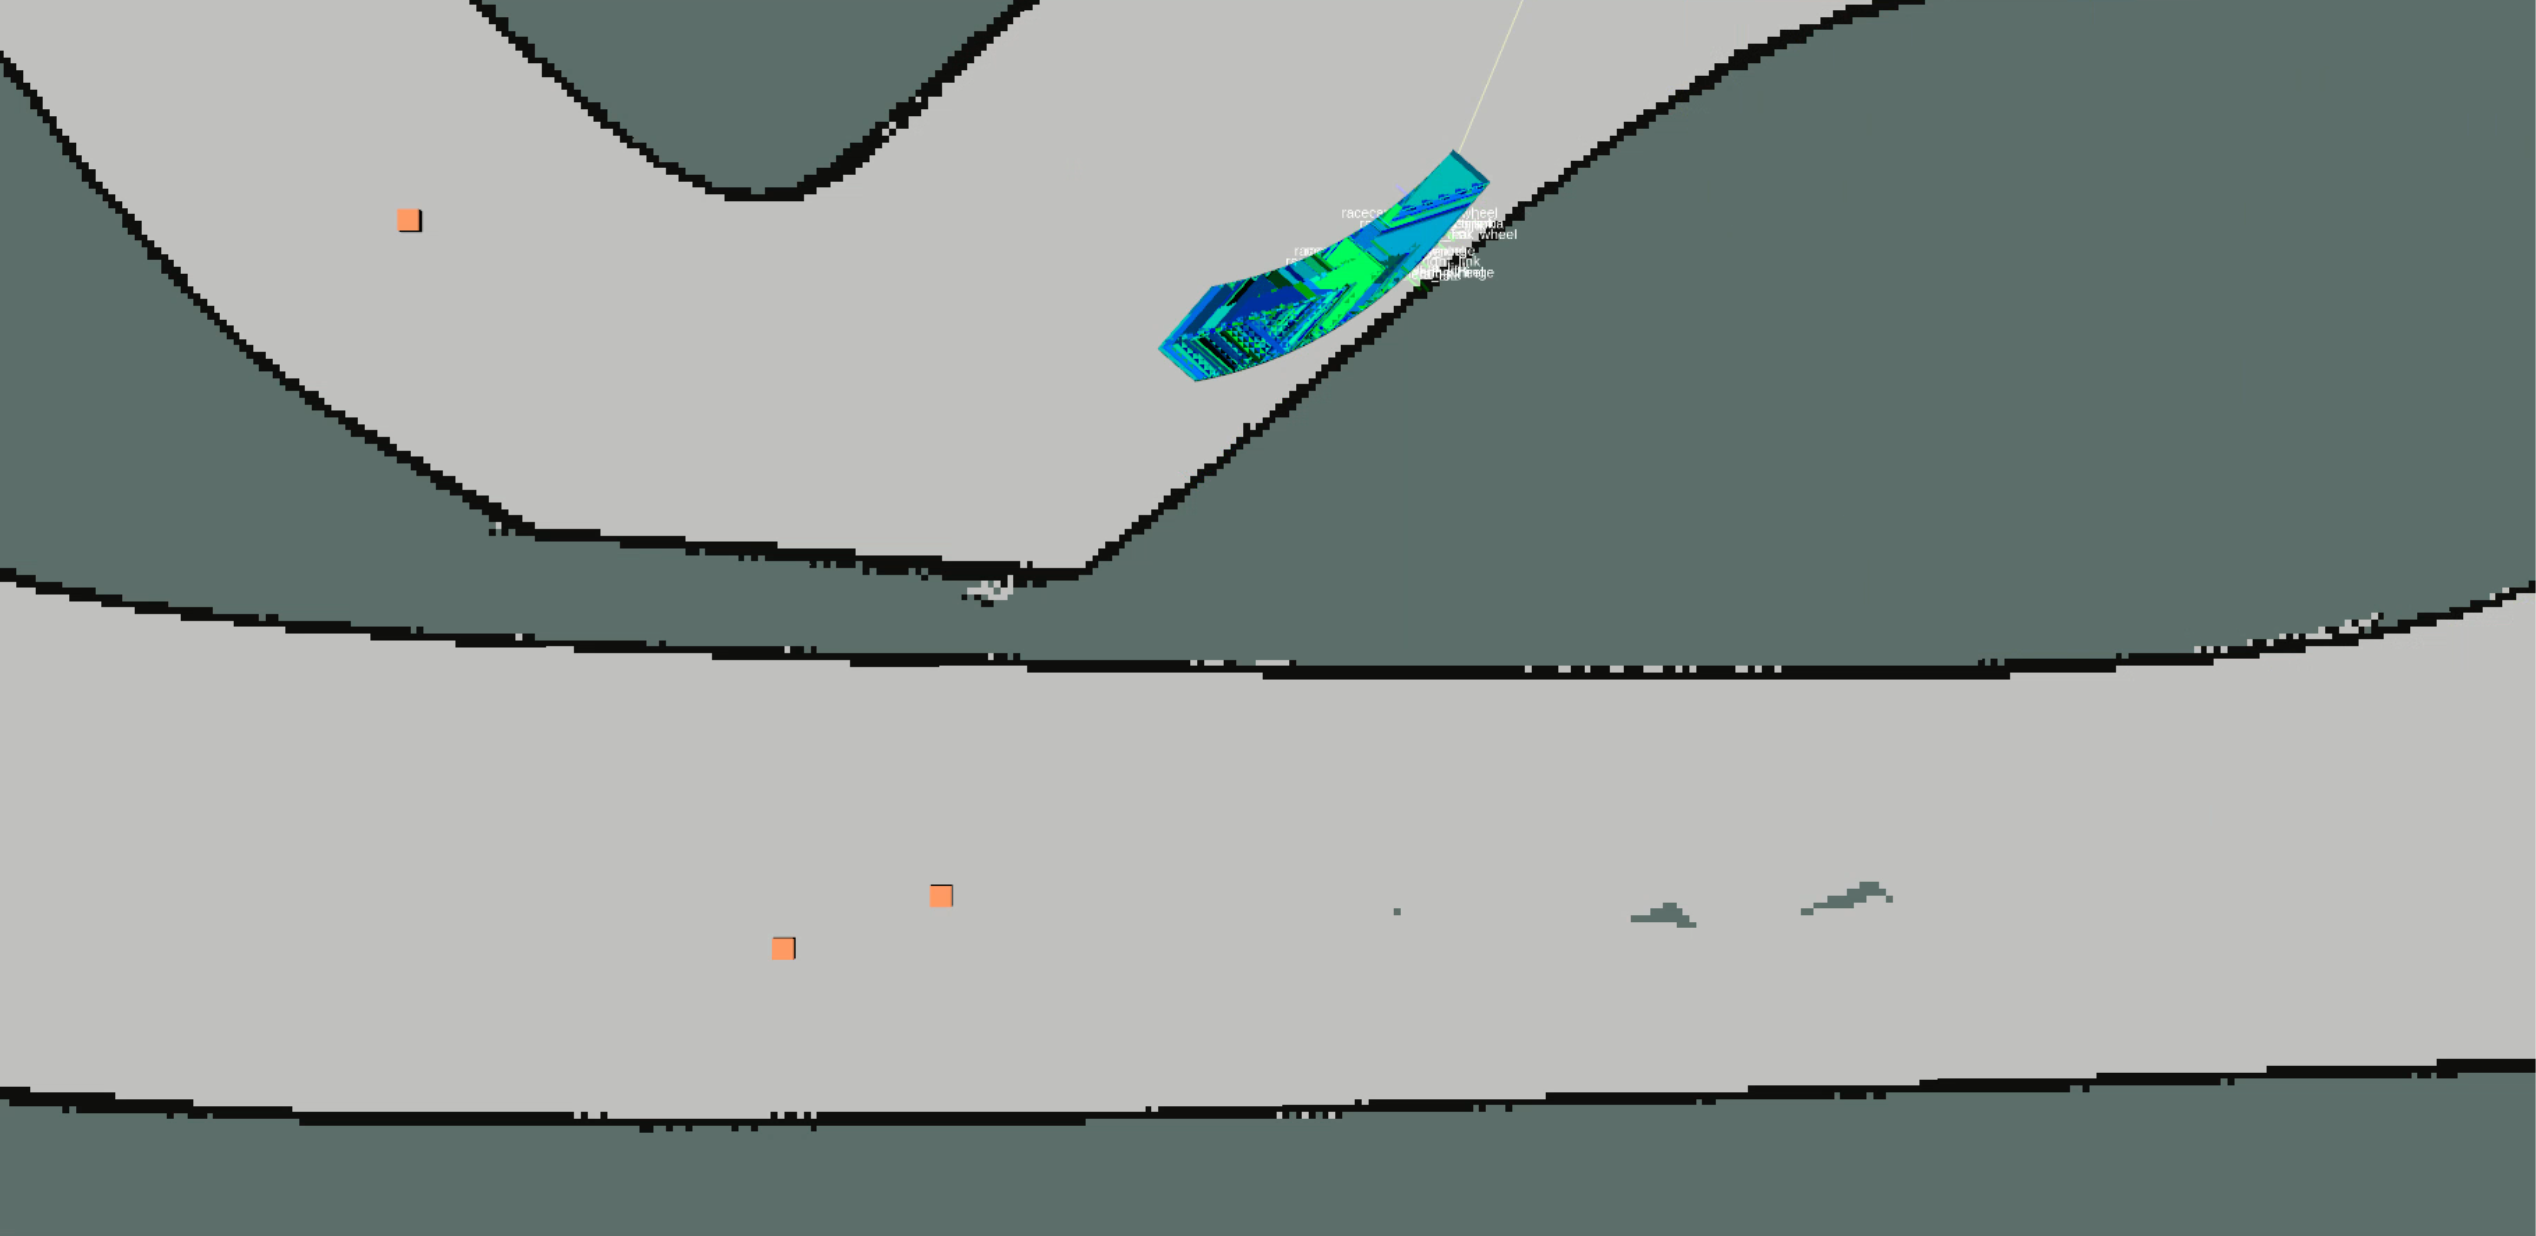
\includegraphics[width=0.9\linewidth]{figures/reach_vis_one.png}
   \caption{Visualization of the set of reachable states using the current control action. This example corresponds to a safe scenario, as there is no intersection with obstacles or the the racetrack walls. The orange squares represent the location of cones and their corresponding bounding box.}
  \label{fig:reachset}
\end{figure}



\section{Experimental Overview}

In order to build and assure the safety of our system at runtime, we perform the following steps. First, we construct a mathematical model of the F1/10 car's physical dynamics using system identification techniques. We then deploy one of our machine learning controllers into the control architecture. These controllers are: (1) Imitation Learning controllers trained to mimic driving behavior using data collected from a series of experimental runs of driving with a baseline controller and (2) Reinforcement Learning controllers (RLc), i.e. a control policy trained using an RL algorithm. The RLcs use lidar sensor information to determine the desired steering angle. At runtime, using the mathematical model that we obtained through system identification and our real-time reachability algorithm, we compute the reachable set of states from the current state and the control input given by our controller, for a specified reach time. During the construction of the reachable set, we perform safety checking in order to gauge whether the reachable set of states intersects with known obstacles or the walls defining the track environment. Lastly, based on the results of the safety checking, we design a simplex strategy to maintain safe operation of the F1/10 model. 

\subsection{The F1/10 Autonomous Platform}

The F1/10 platform proposed by Matthew O'Kelly et al. in \cite{F1102019} was originally designed to emulate the hardware and software capabilities of full scale autonomous vehicles. The platform is equipped with a standard suite of sensors such as stereo cameras, LiDAR (light detection and ranging), and inertial measurement units (IMU). The platform uses an NVIDIA Jetson TX2 as its compute platform, and its software stack is built on the \emph{Robot Operating System} (ROS)\footnote{It is worth noting that ROS is not an operating system in the traditional sense but rather a meta-operating system that primarily provides the message passing interface for various components within robot software development \cite{Huang2014}.} \cite{ROS}. The result is a platform that allows researchers to conduct real-world experiments which investigate planning, networking, and intelligent control on a relatively low-cost, open-source test-bed \cite{F1102019}. Additionally, in order to promote rapid prototyping and consider research questions around closing the simulation to reality gap\cite{Muratore2019}, Varundev Suresh et al. designed a Gazebo-based simulation environment \cite{Gazebo} that includes a realistic model of the F1/10 platform and its sensor stack \cite{varundev_ros_19}. We utilize this simulation environment for a number of experiments and training our controllers.

%\todo{For this version of the paper, we are going to evaluate a whole set of controllers. I can present some of the results from the IL vs RL paper not in the exact same way but just their different efficacies and reachability results}

\subsection{Vehicle Dynamics Model and System Identification}


The physical dynamics of the F1/10 vehicle are modeled using a kinematic bicycle model \cite{Rajamani2012}, which is described by a set of four-dimensional nonlinear ordinary differential equations (ODEs). The kinematic bicycle model is characterized by relatively few parameters and tracks reasonably well at low speeds.\footnote{ The kinematic bicycle model typically tracks well under $5 m/s$ \cite{ivanov2020case}} The model has four states: Euclidean positions $x$ and $y$, linear velocity $v$, and heading $\theta$. The dynamics are given by the following ODEs: 
\begin{align*}
    \Dot{x} & = v\cos(\theta +\beta)\\
    \Dot{y} & = v\sin(\theta + \beta)\\
    \Dot{v} & = -c_av +c_ac_m(u-c_h)\\
    \Dot{\theta} & = \frac{v\cos(\beta)}{l_f+l_r}\tan(\delta)\\
    \beta &= \tan^{-1}\Big(\frac{l_r\tan(\delta)}{l_f+l_r}\Big)
\end{align*}



\noindent where $v$ is the car's linear velocity, $\theta$ is the car's orientation, $\beta$ is the car's slip angle, $x$ and $y$ are the car's position, $u$ is the throttle input, $\delta$ is the steering input, $c_a$ is an acceleration constant, $c_m$ is a motor constant, $c_h$ is a hysteresis constant, and $l_f$ and $l_r$ are the distances from the car's center of mass to the front and rear respectively \cite{ivanov2020case}. For simplicity, since the slip angle is fairly small at low speeds, we assume that $\beta = 0$.
Using MATLAB's Grey-Box System Identification toolbox, we obtained the following parameters for the simulation model: $c_a = 1.9569$, $c_m = 0.0342$, $c_h = -37.1967$, $l_f =0.225$, $l_r = 0.225$. The model was validated using a series of experiments%\footnote{The code used for system identification and model validation can be found at: \url{https://github.com/pmusau17/Platooning-F1Tenth/tree/master/src/race/sys_id}}
with an average \emph{Mean Squared Error} (MSE) of $0.003$. A sample experimental simulation is shown in \ref{fig:validation}. For the hardware platform, we obtained the following parameters: $c_a = 2.9820$, $c_m = 0.0037$, $c_h = -222.1874$, $l_f =0.225$, $l_r = 0.225$, with a validation MSE of $6.75 \times 10^{-4}$.
\begin{figure}[htbp]
  \centering
    % \hspace*{-8mm}  
    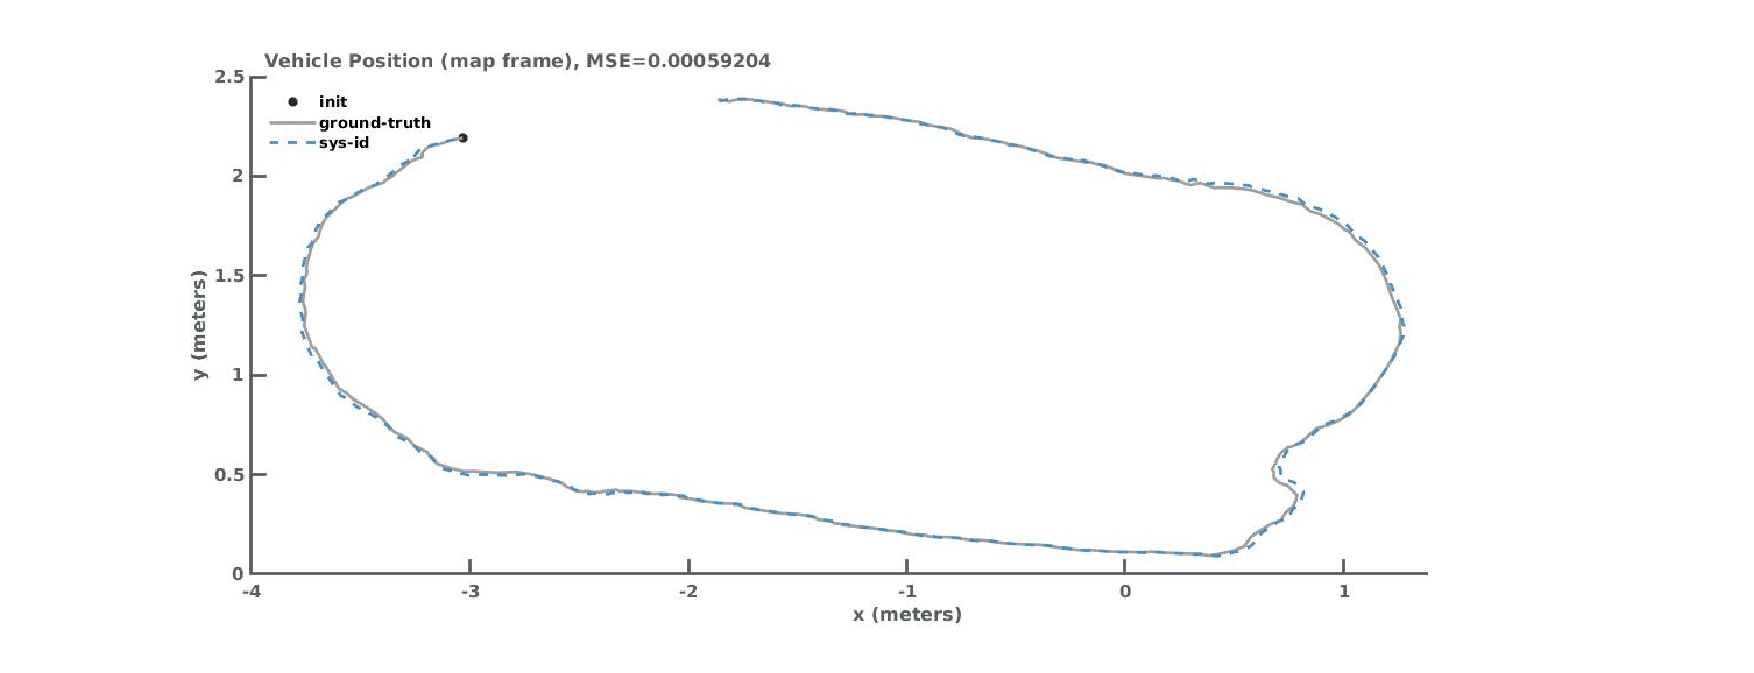
\includegraphics[width=0.8\linewidth]{figures/validation_em.pdf}
   \caption{Model validation for the F1/10 Hardware Model using data collected from a manual set of experimental runs. \emph{Init} corresponds to the starting position of the vehicle in the considered experiment.}
  \label{fig:validation}
\end{figure}
\noindent 



%In order to build and assure the safety of our system at runtime, we perform the following steps. First, we construct a mathematical model of the F1/10 car's physical dynamics using system identification techniques. We then deploy one of our four trained machine learning or \emph{learning enabled controllers} (LECs) into the control architecture. These controllers are: two Imitation Learning controllers (IL) designed to mimic nominal driving behavior from data collected from a series of experiments of driving the vehicle manually, and two Reinforcement Learning controllers (RLc) that synthesize control policies through trial and error. At runtime, using the mathematical model that we obtained through system identification and our real-time reachability algorithm, we compute the reachable set of states from the current state and the control input given by our LEC, for a specified reach time. During the construction of the reachable set, we perform safety checking in order to gauge whether the reachable set of states intersects with known obstacles or the walls defining the track environment. Lastly, based on the results of the safety checking, we design a simplex strategy to maintain safe operation of the F1/10 model. 

\section{Controller Construction}

Modern data-driven or machine learning methods have become increasingly scalable and efficient, and these methods will continue to be deployed in more and more contexts. In this section, we provide a high-level introduction into imitation learning and reinforcement learning and describe the construction of the complex controllers used within our simplex architecture.

\subsection{Imitation Learning}

Imitation learning seeks to reproduce the behavior of a human or domain expert on a given task \cite{Hussein2017ImitationL}. These methods fall under the branch of \textit{Expert Systems} in AI which has seen a surge in interest in recent years. The increase in demand for these approaches is spurred on by two main motivations. (1) The number of possible actions needed to execute a complex task is too large to cover using explicit programming. (2) Demonstrations show that having prior knowledge provided by an expert is more efficient than learning from scratch \cite{Hussein2017ImitationL}.

One of the most common methods for imitation learning is \textit{Behavioral Cloning}, whereby a controller is constructed by learning a mapping from sensor-action pairs collected either from a baseline controller or through human-in-the-loop control. 
%This paradigm was first introduced to train a multilayer perceptron tasked with enabling a modified van to navigate paths at speeds of up to 20 miles an hour \cite{pomerleau1989alvinn}. The work was later replicated with a convolutional neural network architecture in \cite{bojarski2016end} with great success. 
In this work, we utilize behaviour cloning to train two neural network controllers to produce steering angles from sensor inputs. The first controller is trained on camera-images and falls within the class of \textit{end-to-end learning}. The second controller utilizes a much smaller neural network model and is trained on a discrete sampling of lidar distance measurements.%\todo{Our hypothesis is that controllers trained on images will experience greater challenges in zero-shot policy transfer? Maybe not a hypothesis but it would be an interesting result from our analysis}

\subsubsection{End-to-End Learning}
\diego{Isn't the lidar behavior cloning and E2E controller too? End to end means that the output of the controller is solely based on the inputs from the sensors/environments, right?. I would change the name of this subsection. And I guess RL (in this sense) it is also E2E.}
Vision-based perception systems for autonomous driving can be broadly classified into two categories: mediated-perception approaches and end-to-end, or behavioral-reflex, approaches \cite{DeepDrive2015}. Mediated perception approaches involve multiple sub-components for recognizing objects relevant to the driving task, that are then combined into a world representation utilized by a decision manager to issue control actions. In contrast, end-to-end approaches compute a direct mapping from images to control actions \cite{DeepDrive2015}. While end-to-end approaches have proven to be an elegant and effective reduction of a complex system, they are "black box" in nature which makes them difficult to debug. Within the context of this manuscript, we opted to use end-to-end approaches because of their straightforward incorporation within the simplex architecture, and they allow us to evaluate our safety regime more plainly.

%Such systems are typically constructed using data where a human, or baseline controller, controls the system during a series of experiments. The control commands and corresponding images are then used to train a convolutional neural network to fit this non-linear mapping \cite{DirectPerception2019,AlexNet2012}. 

% Mediated-perception approaches involve multiple independent components for detecting objects relevant to the driving task such as lanes, objects, traffic lights, pedestrians, and other vehicles. Each component then returns its observations to a decision manager that controls the vehicle.

% Accordingly, given unexpected behavior, it is hard for the designer to find the source of errant behavior \cite{VisionBased2019}.


%End-to-end approaches have demonstrated efficacy in simple tasks such as lane following, and although they represent an elegant idea, these approaches struggle to be robust in complex traffic and driving scenarios  \cite{DeepPiCar2017}. While mediated approaches are more transparent, making them more accessible to inspection and debugging, end-to-end methods are largely ``black-box'' in nature. Thus, current state-of-the-art systems typically make use of mediated approaches in autonomous vehicle applications. However, these systems exhibit considerable complexity as it relates to the perception problem by detecting redundant objects that may not be useful in driving control decisions \cite{DeepDrive2015}. 

Since the seminal work of Alex Krizhevsky et al. \cite{AlexNet2012} in the ImageNet Large Scale Recognition Challenge, \emph{Convolutional Neural Networks} (CNNs) have revolutionized the field of computer vision. For this reason, we selected such an architecture for our experiments. The CNN utilized within this work is the DAVE Architecture that was utilized by Nvidia to control a 2016 Lincoln MKZ in a series of successful tests \cite{bojarski2016end}. The data we used to train this network was collected from set of simulation experiments where the sensor-action pairs were generated by a path tracking controller optimized to keep the F1/10 in the center of the track. Such an environment is shown in Figure~\ref{fig:racetrack}. The path-tracking controller was designed using the well-known pure-pursuit algorithm \cite{coulter1992implementation}. To ensure robustness, we augmented these experiments with a set of configurations in which the F1/10 deviated from the center of the track, and recorded the actions that the path tracking controller enacted to return to the nominal path. In sum, the dataset consisted of 5000 images.  To investigate the use of our simplex architecture in novel contexts, the training data was collected in the absence of obstacles.

\begin{figure}[!htbp]
  \centering
    % \hspace*{-8mm}  
    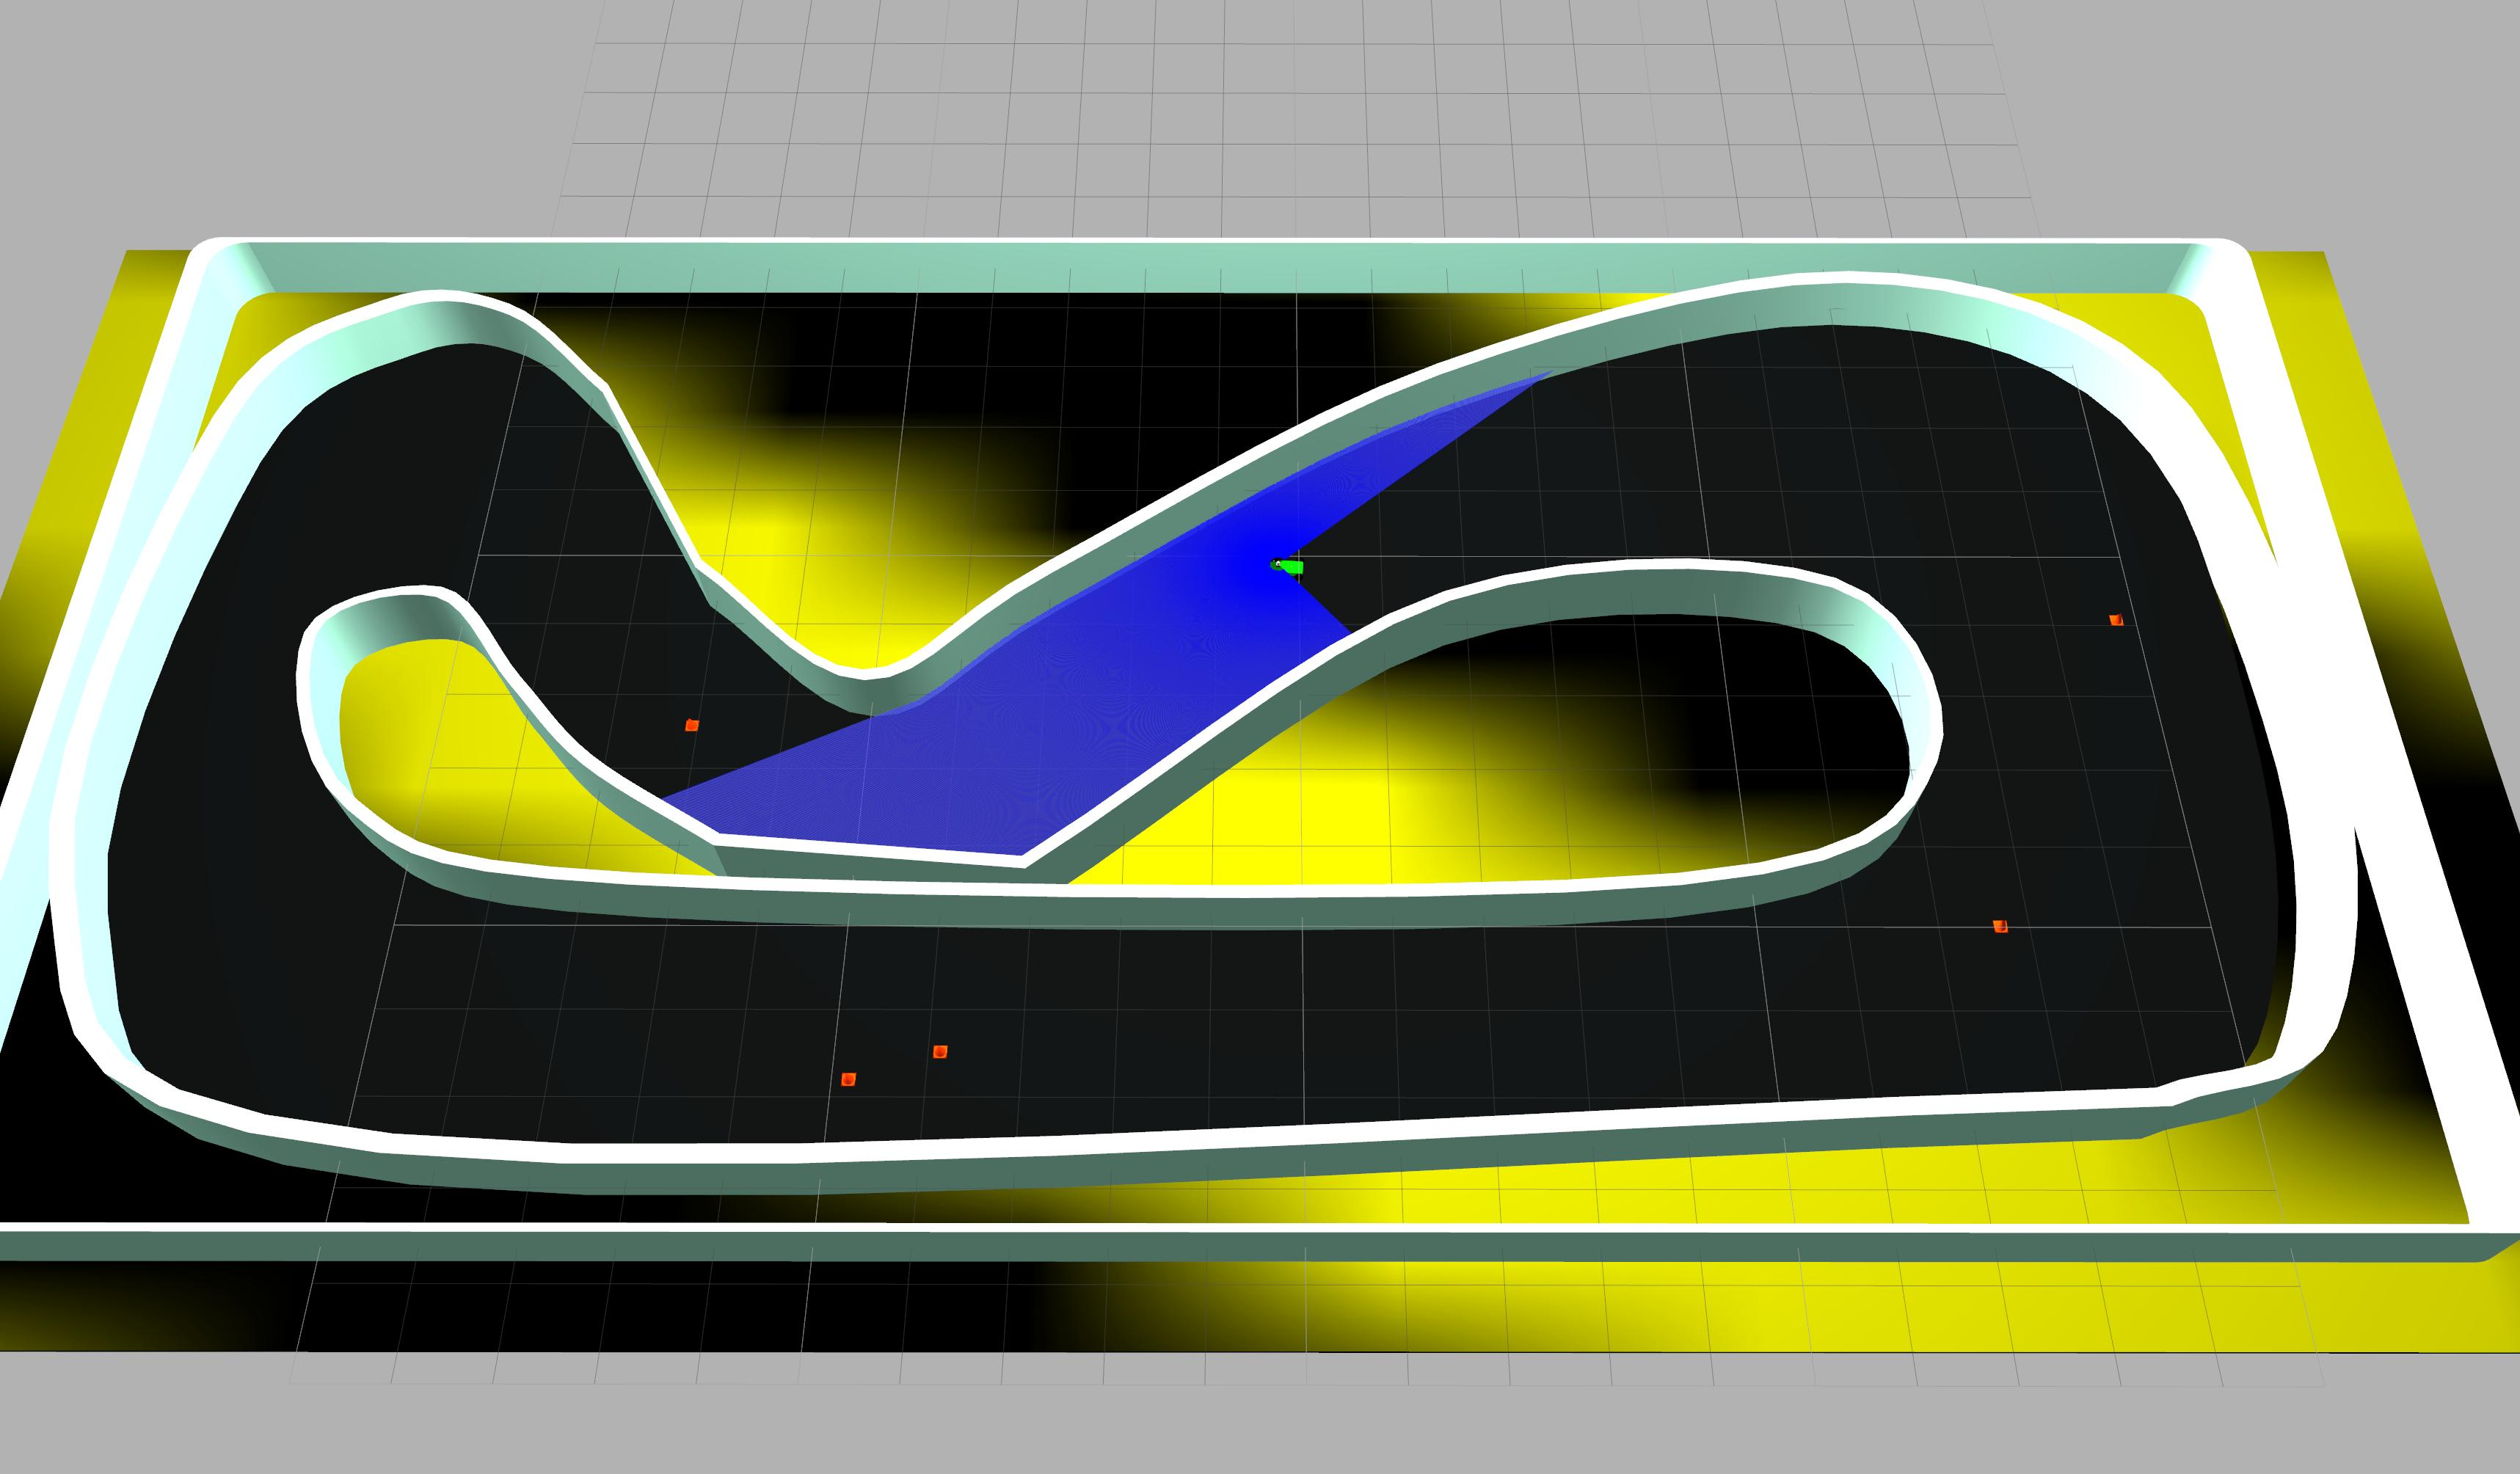
\includegraphics[width=0.7\textwidth]{figures/gazebo.jpg}
   \caption{Simulation of F1/10 Car and obstacles using Gazebo.}
  \label{fig:racetrack}
\end{figure}

\subsubsection{Lidar Behavioral Cloning}
\label{sec:lidar cloning}
The second network considered for behavioural cloning was a standard multi-layer perceptron network that consisted of an input layer 2 fully connected hidden layers of 64 nodes with ReLU activation functions, and a fully connected output layer with a $\tanh$ activation function. The input layer accepts nine range values collected from the LiDAR at $-90^{\circ}$, $-60^{\circ}$, $-45^{\circ}$, $-30^{\circ}$, $0^{\circ}$, $30^{\circ}$, $45^{\circ}$, $60^{\circ}$, and $90^{\circ}$ from forward. The range values are clipped between $[0m, 10m]$. The data used to train this controller was collected in the same fashion as the end-to-end regime. 


%We divided the driving task into five distinct categories based on the images observed from our on-board camera. The classes we utilized are: left, weak left, straight, right, and weak right. The classes are displayed in \ref{fig:classes}. The corresponding control inputs are ($\delta = 0.51$), ($\delta = 0.10$), $(\delta = 0.0)$, ($\delta=-0.51$), and ($\delta= -0.10$) respectively.

%\begin{figure}%[ht]
%  \centering
%    % \hspace*{-8mm}  
%    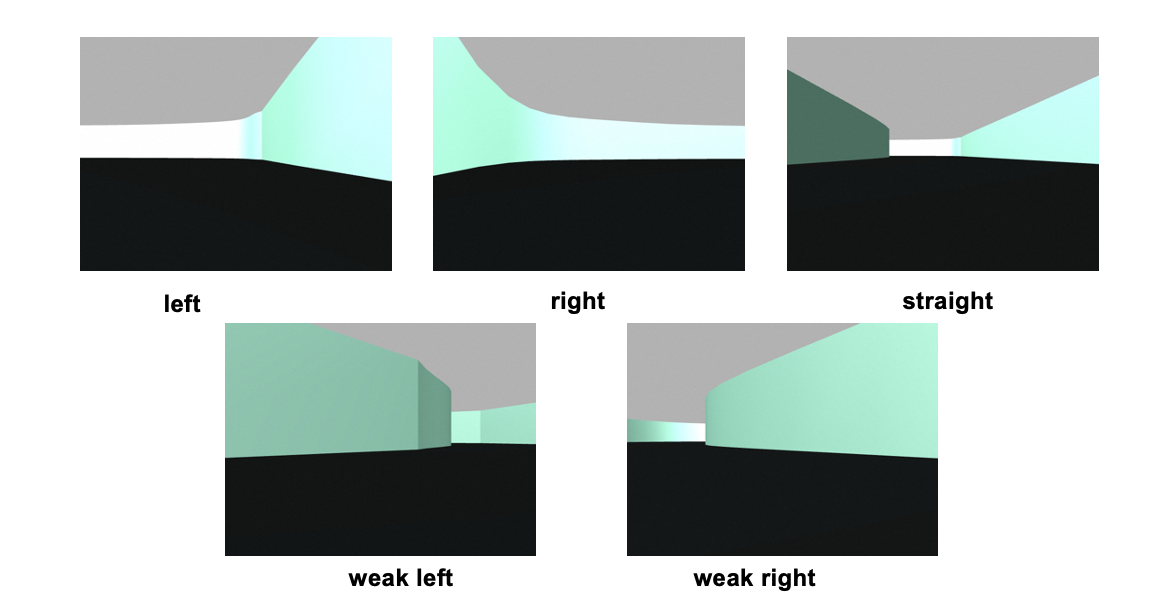
\includegraphics[width=0.7\linewidth]{figures/classes.png}
%   \caption{Classes used in the the end-to-end classification task.}
%  \label{fig:classes}
% \end{figure}

 %\url{https://github.com/pmusau17/Platooning-F1Tenth/tree/master/src/computer_vision}}.
%Additionally, in order to investigate the use of our simplex architecture in novel contexts, the neural network was trained in the absence of obstacles within the racetrack environment.



\subsection{Reinforcement Learning Control}
Reinforcement Learning and Deep Reinforcement Learning (both referred to as RL) have become increasingly popular for training Neural Network controllers to achieve state-of-the-art performance on many high-dimensional control tasks \cite{lillicrap2015continuous, schulman2017proximal, mania2018simple, haarnoja2018soft}. Despite the growing success, controllers trained using RL are not widely seen in real-world systems due to the limitations highlighted in \cite{dulac2019challenges}. \diego{I mention a few of the limitations and then refer the reader to that paper for a detail discussion of the challenges.} Instead, RL's success remains primarily within simulation. Additionally, moving the trained control policies from simulation to the real world, \emph{sim2real}, often results in undesired, poor, and/or dangerous behavior \cite{jang2019ICCPS, kadian2019we}.

In this manuscript, we highlight how using this simplex architecture can prevent dangerous behavior when transferring a trained policy from simulation to the real world or to a different simulated environment.
To demonstrate the effectiveness of this method, we trained  two well-known state-of-the-art reinforcement learning algorithms, an off-policy deep reinforcement learning algorithm known as \emph{Soft-Actor-Critic} (SAC), \cite{haarnoja2018soft}, and an on-policy RL algorithm, known as \emph{Augmented Random Search} (ARS), \cite{mania2018simple}. %The policies were trained in our simulator with hyperparameters listed in Appendix \ref{app:rl_training}.
In line with the imitation learning experiments, the agents were trained on the racetrack shown in \ref{fig:racetrack} with no obstacles and no backup controller. After training to an optimal policy\footnote{We plan on participating in the artifact evaluation by submitting the source code and experiments that enabled this work.}, the control policies were locked and used without any further augmentations for the experiments described in Section \ref{sec:experiments}. This method of locking the control policy and using it in a different environment without further augmentations is often referred to as \emph{zero-shot policy transfer}.

% \subsubsection{Augmented Random Search}
\subsubsection{Augmented Random Search} 
(ARS) was first proposed in 2018 as a random search method for training static, linear policies for continuous control problems \cite{mania2018simple}. Their simple method was able to match state-of-the-art sample efficiency on the benchmark MuJoCo locomotion tasks\footnote{These benchmark tasks are described in more detail at \url{https://gym.openai.com/envs/\#mujoco}}, demonstrating that deep neural networks might not be necessary for some complex control tasks. We chose to highlight this RL algorithm because in comparison to algorithms such as Proximal Policy Optimization (PPO) \cite{schulman2017proximal} or Soft Actor-Critic (SAC) \cite{haarnoja2018soft}, ARS can achieve optimal results with simpler reward functions. Successfully training a PPO or SAC agent often requires considerable reward shaping or the use of a gate-based reward that is more difficult to construct within the simulation environment.

The output control signal of the policy, $\delta = \pi(s)$, is the desired steering angle clipped between $\pm 34^{\circ}$. The input, $s$, consists of $271$ lidar range values collected from between $\pm90^{\circ}$ from forward. The lidar values are clipped between $[0, 10]$ to limit the impact of larger range values.

\subsubsection{Soft Actor Critic (SAC)}
The SAC controller was trained
%using hyper-parameters given in\ref{app:rl_training} and utilized 
using the architecture described in Section~\ref{sec:lidar cloning}. The agent optimizes performance on on a dense reward function that assigns a positive reward for counterclockwise progress around the track. The reward is calculated using a reference path that runs through the middle of the track. The value of the reward is the positive arclength between the previous closest point and the current closest point along the path. This reward function encourages the agent to complete as many laps as possible as quickly as possible. During the training process, we halted the simulation to evaluate the agents performance after 500 training steps. The performance is measured by how many laps the agent can complete within 100 seconds. This is more than enough time to complete 2 laps in the training track. The evaluation is repeated up to 10 times and training stops when the agent is able to complete at least 2 laps 10 times in a row. Once the agent is able to complete at least 2 laps 10 times, the training process is halted and control policy is saved for our experiments.


% The control policy uses the forward-facing semi-circle of collected lidar range data to determine the desired steering angle by way of a linear policy, i.e. a weight matrix. 
\section{ONLINE REACHABILITY COMPUTATION}

Before outlining the algorithm, let us define two key terms relevant to our approach.\smallskip

\begin{definition}%
(REACHTIME). The reachtime, $T_{reach}$, is the finite time horizon for computing the reachable set.
\end{definition}%\smallskip
\begin{definition}%
(RUNTIME). The runtime, $T_{runtime}$, is the duration of (wall) time the algorithm is allowed to run.
\end{definition}% \smallskip

With that, the real-time reachability algorithm works as follows. Using the dynamics model obtained for the F1/10, the crux of the real-time reachability algorithm is computing the set of reachable states from the current time $t$ up until $(t+T_{reach})$, where $T_{reach}$ represents the reachability horizon. The algorithm utilized within this work is based on mixed face-lifting, which is part of a class of methods that deal with \textit{flow-pipe construction} or \textit{reachtube computation} \cite{Johnson2016}. This is done using snapshots of the set of reachable states that are enumerated at successive points in time. To formalise this concept, we define the reachable set below.
\smallskip
\begin{definition}%
(REACHABLE SET). Given a system with state vector $\textbf{x}(t) \in \mathbb{R}^n$, input vector $\textbf{u}(t) \in \mathbb{R}^m$, and dynamics $\dot{\textbf{x}}(t)=f(\textbf{x}(t),\textbf{u}(t))$, where $t$ is time, and the initial states $\textbf{x}_0 = \textbf{x}(0)$ and inputs $\textbf{u}_0 = \textbf{u}(0)$ are bounded by sets, $\textbf{x}_0 \in \chi_0$, $\textbf{u}_0 \in \mathnormal{U}$. The reachable set of the system for a time interval $ t \in [0,T_{reach}]$ is:%
%
\begin{equation*}%
    \mathnormal{R}_{[0,T_{reach}]} = \big \{ \psi(\textbf{x}_0,\textbf{u}_0,t) \ \big| \ \textbf{x}_0 \in \chi_0, \ \textbf{u}_0 \in \mathnormal{U}, \ t \in [0,T_{reach}\big]\},%
\end{equation*}%
%
\noindent where $\psi(\textbf{x}_0,\textbf{u}_0,t)$ is the solution of the ODE at time $t$ with initial state $\textbf{x}_0$ under control input $\textbf{u}_0$.
\end{definition}%
\smallskip

In general, it is not possible to obtain the exact reachable set $\mathnormal{R}_{[0,T_{reach}]}$ \diego{There is a paper that formally reasons that computing the exact reachable set of nonlinear systems (bycicle model) is NP-hard... I could try to find it if we want to cite it, although not sure how important it is for the runtime verification since even if it was possible, it would be too computationally expensive to use it in this regime}, so we compute an over-approximation such that the actual system behavior is contained within the over-approximation \cite{Lin2020}. The algorithm utilized in this work utilizes $n$-dimensional hyper-rectangles (``boxes'') as the set representation to generate reachtubes \cite{Johnson2016}. Over long reach-times, the over-approximation error resulting from the use of this representation can be problematic. However, for short reach-times it is ideal in terms of its simplicity and speed \cite{Bak2014}.


The over-approximation error can be controlled by a step size, $h$, used to discretize the time interval defined by the reach horizon. In designing the technique, Bak et al. leveraged this step size in order to tune the over-approximation error as well as the runtime, $T_{runtime}$, associated with computing the reachable set. In doing so, the approach becomes amenable to the anytime computation model in the real-time scheduling literature \cite{Liu1991}.


Thus, given a fixed runtime (wall-time), we compute the reachable set $\mathnormal{R}_{[0,T_{reach}]}$, using an initial step size, $h$, and if there is remaining runtime once this computation completes, the computation is restarted with a smaller time step. In this work, we decrease the step size by half in each successive iteration. A high level overview is presented in Algorithm~\ref{alg:algo_rtreach}, and we refer readers to the following papers for an in depth treatment of these procedures \cite{dang2000,Bak2014,Johnson2016}. The relationship between the over-approximation error and the step size can be seen in Figure \ref{fig:reach_refine}.

\begin{algorithm}[]%
\DontPrintSemicolon 
INITIALIZE{
\\
\textbf{Input:} $\chi_0,\mathnormal{U},T_{reach}, T_{runtime}$ \\
\textbf{Output:} safe (boolean)
}

\vspace{2mm}

REACHABILITY ANALYSIS\\
$elapsedTime = 0$\;
\While{elapsedTime $<T_{runtime}$} {
    %\% Construct the Reachable Set\;
    safe = true\;
    $\mathnormal{R}_{[0,T_{reach}]}= constructReachSet(\chi_0,\mathnormal{U},T_{reach},h)$\;
    %\% Check for intersections with unsafe set\;
    \If{$\mathnormal{R}_{[0,T_{reach}]} \cap \Lambda \neq \emptyset $}{
    safe = false\;
    }
    $elapsedTime$ = computeElapsedTime()\;
    $h = h /2$\;
    
    
    
}
\textbf{return:} safe
\caption{Real-time Reachability Algorithm}
\label{alg:algo_rtreach}
\end{algorithm}%



\begin{figure*}[htbp]%[tb]
  \centering
  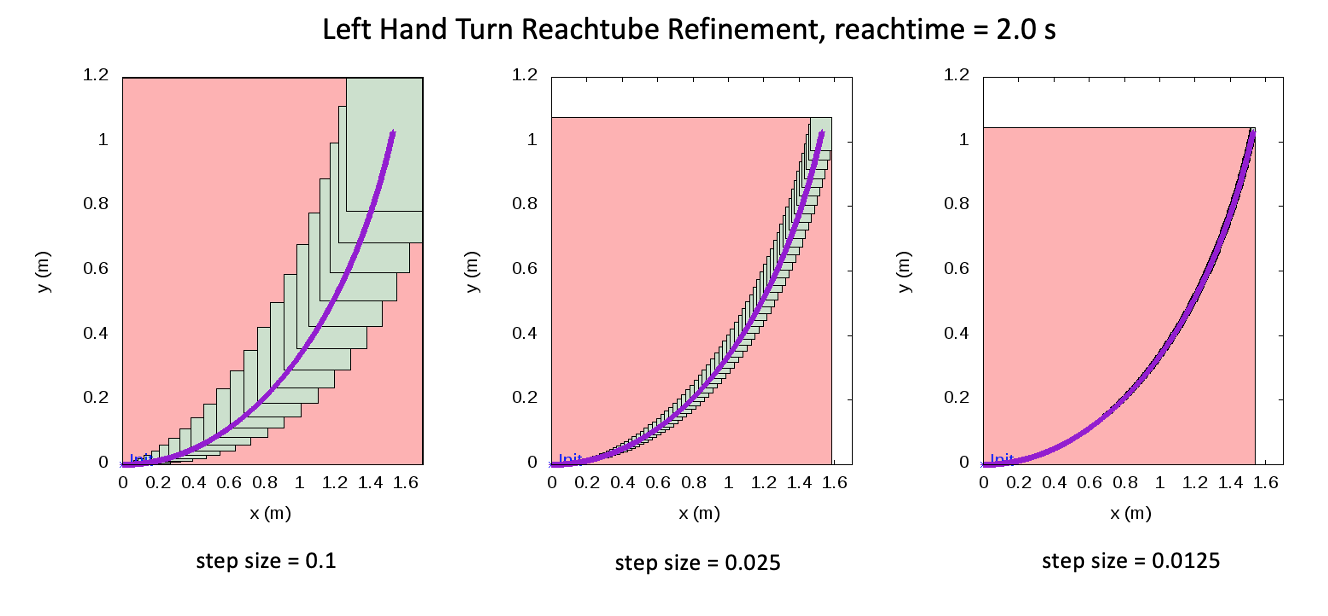
\includegraphics[width=\linewidth]{figures/refinement_reachset.png}
  \caption{The real-time reachability algorithm always returns an over-approximation of the reachable set of states. The over-approximation error decreases with successive iterations, provided that there is enough runtime for re-computations. The above images demonstrate this aspect by simulating a left hand turn control action for a reachtime of two seconds. The green boxes represent the set of reachable states, the red rectangle represents the interval hull of the reachable states, and the purple points are points obtained from a simulation of the vehicles physical dynamics.}
  \label{fig:reach_refine}
\end{figure*}%


% Furthermore, by supposing a dynamics model for the dynamic obstacles within the environment, one can reason about potential future collisions.

\section{SAFETY CHECKING}
The computation of the reachable set allows us to reason whether the system under consideration will enter an unsafe situation in the future. Safety checking is then formulated as checking whether an intersection between a set of unsafe states and $\mathnormal{R}_{[0,T_{reach}]}$ is empty. Let $\Lambda$ represent the set of unsafe states.\smallskip

\begin{definition}%
(SAFETY). A system is considered safe over the finite time horizon, $T_{reach}$, if  $\mathnormal{R}_{[0,T_{reach}]} \  \cap \ \Lambda \ = \ \emptyset$.
\end{definition}%\smallskip
%
%Here, $\Lambda$ consists of the static obstacles within the environment. %\textcolor{blue}{Diego --- Don't think this last sentence (in blue) is necessary. --- We formalize this concept below.} \smallskip

\begin{definition}%
(UNSAFE SET). The unsafe set,  $\Lambda$, consists of all static obstacles within the environment and the boundaries of the racetrack.
\end{definition}%

\diego{How are these boundaries represented? Are they exact / over-approximation representations?}
%Given a set of $N$ dynamic obstacles, and a set $O$ of static obstacles within the environment, let $\mathnormal{R_i}_{[0,T_{reach}]}$ denote the reachable set of the $i$-\textit{th} dynamic obstacle. The set of unsafe states $\Lambda$ is:
%\begin{equation*}
%    \Lambda \ = \ O \ \cup \ \bigcup\limits_{i=1}^{N} \ \mathnormal{R_i}_{[0,T_{reach}]}.
%\end{equation*}
%\end{definition}\smallskip

There are two key parameters that play a major role in safety checking. The first parameter is the finite time horizon, $T_{reach}$, over which we are reasoning about safety. The second parameter is the amount of time, $T_{runtime}$, allocated for the computation of the reachsets. In our experiments we utilized a reach time of 1.0 $s$. This was determined by empirical determinations of how long it took the F1/10 to come to a stop at speeds less than $1.5 m/s.$\footnote{The selection of velocities below 1.5 $ms$ was due to the size of our physical track that was ~13.08 meters in length. Races held by the F1/10 community are around typically 30-50 meters in length with large distances between the track walls.} The runtime allocated for the reachability algorithm was set at 25 $ms$ so as to ensure execution within a 20 $Hz$ control period. In the experiments that follow, we provide insight on how the wall-time impacts safety declarations. 

Finally, rather than computing the reachable set of states first, and then checking whether or not the system has entered an unsafe scenario, the reachability algorithm we utilize does the checking during the computation with the intermediate hyper-rectangles. This prevents us from needing to dynamically store the reachable set and allows for further checks at each level of refinement. If an unsafe state is encountered, then the computation can recommence and determine whether or not the unsafe declaration is overly conservative.

%\subsection{Dynamic Obstacle Model}

%The obstacle tracking problem is a well studied and challenging topic within the autonomous vehicle, computer vision, and robotics literature \cite{YilmazObjectTracking}. Typically some assumptions are required in order to constrain the tracking problem to best suit the context of the application. In our framework we assume that the obstacles are described by a two dimensional kinematic model and a corresponding bounding box. The equations describing the ODE are given as follows: 
%
%\begin{align*}%
%    \Dot{x} & = v_x,\\%
%    \Dot{y} & = v_y,%
%\end{align*}%
%
%\noindent where $v_x$ and $v_y$ are the velocities in the x and y direction respectively. Additionally, we make the assumption that we have access to the position and velocity of the other race participants. The use of a multi-object tracking approach is left for future work.

\section{ROS Simplex Architecture}



\label{section:simplex}
The simplex architecture for the F1/10 is designed using ROS \cite{ROS}, and an overview of this design is shown in Figure~\ref{fig:simplex_arch}. Within this architecture, the primary sensors we rely on are a LiDAR and Stereo Labs' Zed Depth Camera. The messages from the LiDAR are published at $40 \ Hz$, and the Camera messages are published at $20 \ Hz$. Additionally, we rely on odometry information, published at $40 \ Hz$, in order to accurately ascertain the state of the F1/10 vehicle. In our design, we decouple the control of the car's steering and throttle control. The steering control, $\delta$, is governed by our learning-based controller, and the throttle control is designed to maintain a constant speed, $u$, when the learning-based controller is in use. 

The publishing rate of the decision manager within the simplex architecture is limited by the on-board camera, which captures images at 20 frames-per-second (FPS)\footnote{On the hardware platform, the camera can capture images as fast as 100 FPS. However, to keep the experiments consistent we limited the FPS to 20 FPS.}. Thus, as mentioned previously, we limited $T_{runtime}$, to $25 ms$ which corresponds to half the length of a control period. This was chosen based on empirical observations of the average execution time of the reachability algorithm, as well as a desire to ensure that the other parts of the decision logic could be successfully processed within a single control loop.

\begin{figure}[htbp]%
  \centering
  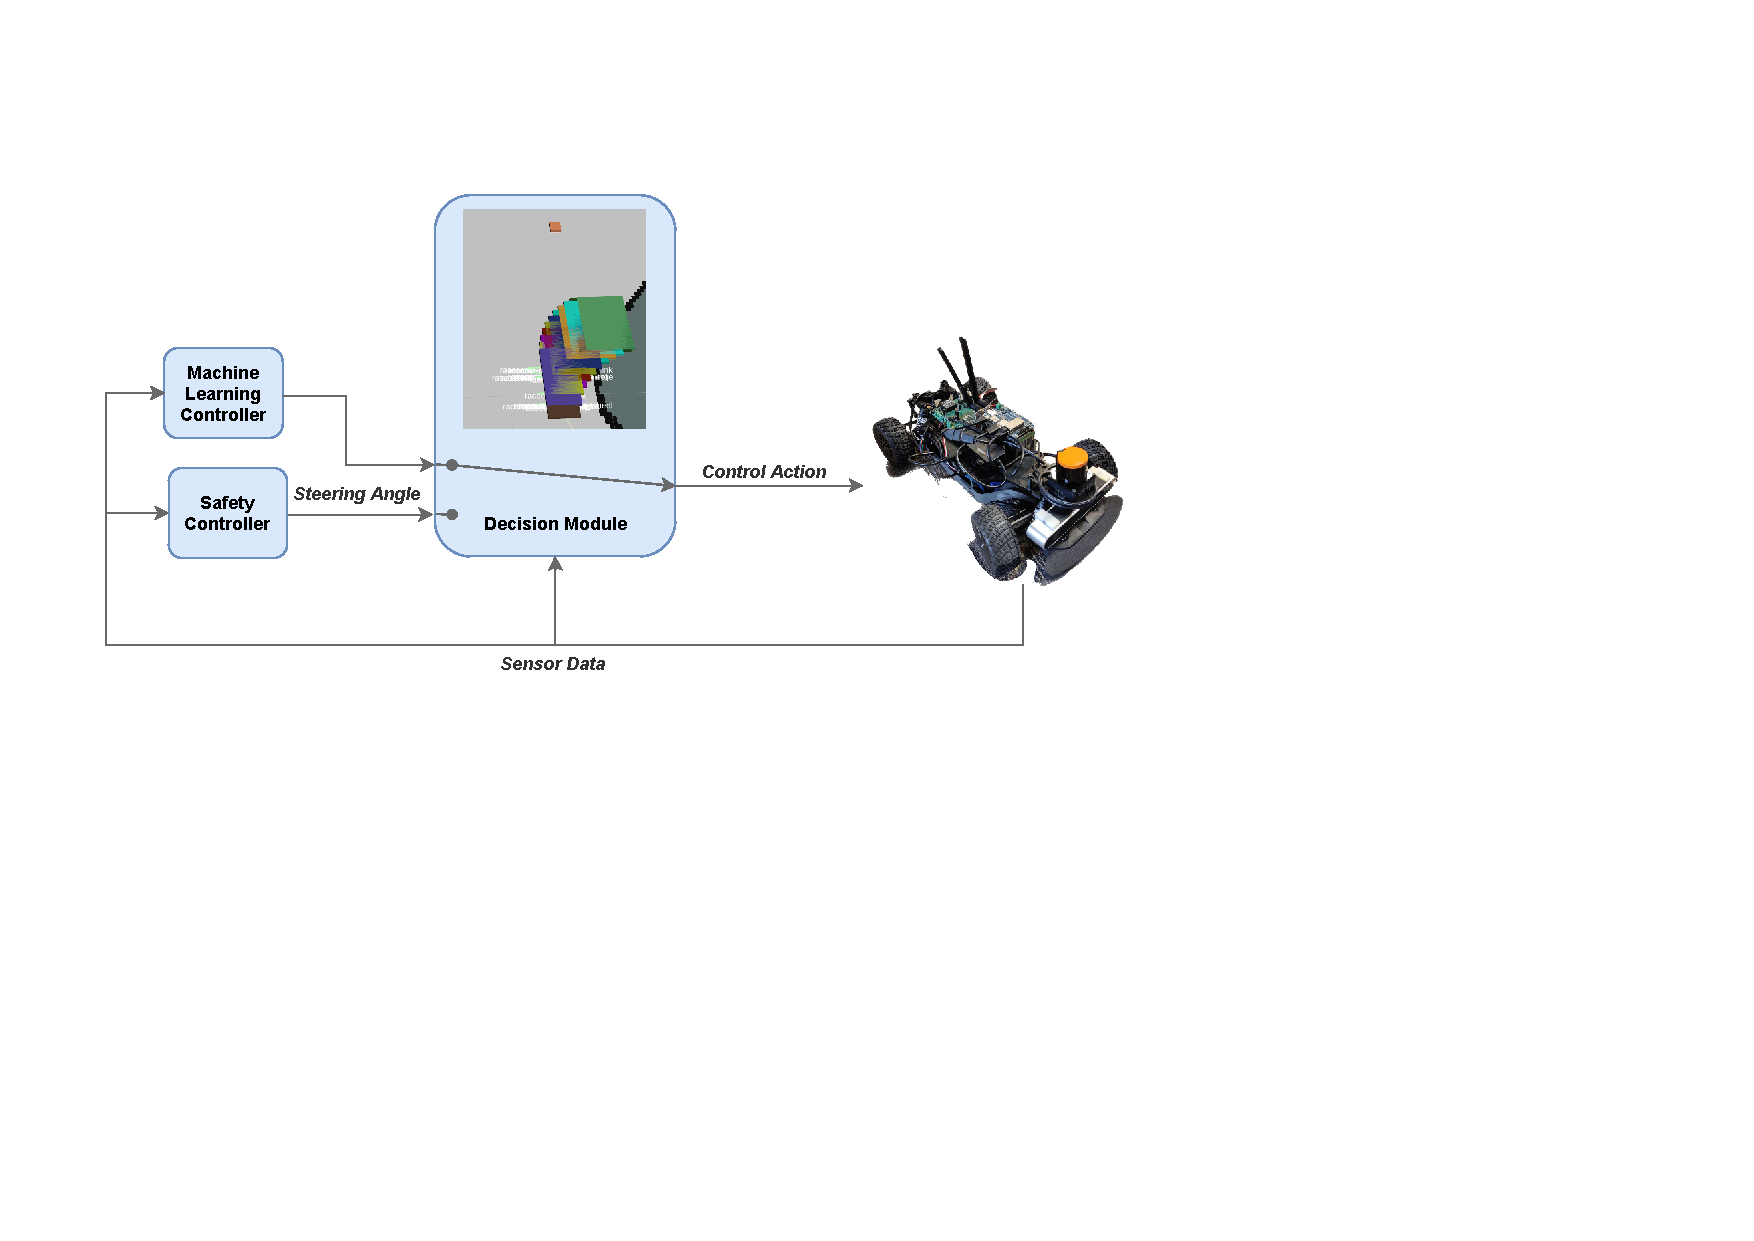
\includegraphics[width=0.7\linewidth]{figures/simplex_simple_v2.pdf}
  \caption{Overview of the Simplex architecture deployed on the F1/10 System as described in Section \ref{section:simplex}. The switching logic consists of monitoring the intersection between the F1/10 reachable set and the positions of static obstacles within the environment.}
  \label{fig:simplex_arch}
\end{figure}%

%\todo{Look into this a little more. See if I can come up with a more compelling justification }

In the traditional simplex architecture, for the system to be verified as correct, both the decision module and the safety controller must be verified \cite{Mehmood2021}. While this is straightforward for relatively simple controllers, it is significantly more challenging for many classes of controllers \cite{ivanov2020case}. Especially, when real-time execution is considered. In light of this, we opted not to develop a ``formally verified'' safety controller as is typically used within the simplex architecture. Instead, we selected a controller based on a gap-following algorithm optimized to avoid collisions with obstacles. A detailed description of the gap-following algorithm can be found in the following report \cite{otterness_2019}. It was primarily selected due to its robustness \diego{robustness? In what sense?} and simplicity.  Our primary focus was the evaluation of the real-time reachability regime and our future work will consider verification of both the decision module and safety controller. 


\section{Experimental Evaluation}
\label{sec:experiments}
%\todo{Change this for emsoft}
%We evaluated our approach in an autonomous racing context inspired by the F1/10 Autonomous Racing Competition \cite{okelly2020}, where the vehicles are tasked with navigating a structured environment in a head-to-head race\footnote{The rules for the competitions can be found here: \url{https://f1tenth.org/race/rules-v2.pdf}}. During a race, vehicles are penalized for collisions with other race participants and with the track boundaries, and any serious collision results in disqualification. We denote the agent for which we are reasoning about safety as the ego vehicle. 

%During the race, we compute the set of reachable states for the ego vehicle and the other race participants over a finite time horizon. The lidar and stereo-camera are used for localization. The first parameter required by our regime is the finite time horizon over which we are reasoning about safety and in our experiments, this was determined by empirical determinations of how long it takes the F1/10 vehicle to come to a stop at various velocities. The ego vehicle traveled at a constant speed of 1.0 m/s, while the other race participants traveled at a constant speed of 0.5 m/s.\footnote{The selection of velocities was chosen out of a desire to promote interactions between the two vehicles and due to the size of our track that was ~13.08 meters in length. Races held by the F1/10 community are around typically 30-50 meters in length with large distances between the track walls.} A reach-time horizon of one second was determined acceptable to reason about safety for the ego vehicle and 0.8 seconds for the opponents.

%The second parameter required by our regime was the runtime allocated for the computation of the reachsets. Since the reachability regime utilized in this work is anytime in nature, increasing the allocated runtime allows for tigher appromiximations of the reachable set. An in-depth analysis of the reachability regime can be found in \cite{Bak2014}. In our experiments, we selected a wall-time of $10ms$, so as to ensure execution within a control period of $40 \ Hz$. 


% machine with We utilized two different laptop configurations to evaluate the simulation experiments. The first machine was a Dell Precision 7520 with 32GB RAM, an eight-core Intel Core i7-6820HQ CPU $@ 2.70\textrm{GHz}$ processor, and an Nvidia Quadro M2200 4GB graphics card. The second machine was 

Having described the details of our reachability algorithm, controller development, and the simplex architecture construction, we now present the results of our empirical evaluations both in simulation and on the hardware platform. We ran our experiments on platforms running Linux (Ubuntu 16.04 LTS). The simulation experiments were conducted on a Dell XPS-15 (9570) with 32GB RAM, a six-core Intel Core i7-8750 $@ 4.1\textrm{GHz}$ processor, and an Nvidia GeForce GTX 1050Ti 4GB graphics card. The motivation for conducting simulation experiments stemmed from a desire to ensure fair comparisons over a large number of experiments, and to promote reproducibility for those without hardware access.\footnote{We plan on participating in the artifact evaluation by submitting the source code and experiments that enabled this work.} The hardware experiments were done on an Nvidia Jetson-TX2 with a Dual-core Nvidia Denver 64-bit CPU (ARM), a quad-core ARM A57 Complex, and an NVIDIA Pascal Architecture GPU with 256 CUDA cores. The latter configuration validates our claims that our safety architecture admits minimal resource requirements. 


Our evaluation included a sizeable diversity of experiments with respect to the speed set-point utilized by the machine learning controller, $u$, the wall-time utilized by the real-time reachability algorithm, $T_{runtime}$, the presence and configuration of obstacles, and an examination of how each controller performed when transferred to the real-world hardware platform with no additional training. This allowed for an enlightening analysis on the various trade-offs that exist within our safety architecture. For context, the speed and wall-time analysis was evaluated on 48 different combinations of 30 experimental executions. %Due to space limits, we present a summary of those experiments and have included the remaining experiments in Appendix~\ref{app:experiments}. 
In the tables that follow, ML refers to the machine learning controller, SC refers to the safe controller, and std refers to standard deviation. %The simulation results were conducted on the Dell Precision 7520.

\subsection{Simulation}
In the considered simulation scenarios, the F1/10 vehicle is tasked with navigating a racetrack environment that has a number of cones\footnote{For the benchmark experiments, we used six cones.} placed at random locations before the start of the experiment. The locations of the cones are known \emph{a priori}, and Figure~\ref{fig:racetrack} provides a snapshot of this setup. Utilizing the control architecture discussed in Section \ref{section:simplex}, we ran over 1400 simulation episodes with a timeout of 60 seconds each. That is roughly enough time to complete 2 laps at a speed of 1 $m/s$. %Of these simulations, 400 were done with the reinforcement learning controller, and the other 400 were done using the end-to-end controller. 

\todo{There were a few collisions at speeds higher than 1.5 m/s only with the e2e, how do I talk about these.}


For benchmarking purposes, we recorded the mean execution-times (Mean ET)\footnote{The mean execution time was calculated using a cumulative moving average \cite{Jin2019}.} of our real-time reachability algorithm, as well as the average number of iterations utilized in constructing the reachable set (Mean Iters). While typically a discussion of upper bounds on execution times involves a discussion of the worst-case execution time (WCET), we instead report the Mean ET. In general, the WCET is unknown or difficult to derive without the use of static analysis proofs \cite{Reinhard2008}. Since our safety regime relies on ROS, which is highly dynamic and distributed, it is prohibitively difficult to perform an exhaustive exploration of the space of all execution times, and thus derive the WCET.  However, we provide a rough proxy of the WCET by reporting the maximal observed execution times (MOET)  \cite{Reinhard2008} in Table~\ref{tab:additional}. %Lastly, we analyzed what percentage of the time the safety-controller was used during the experiments%\footnote{The benchmarking experiments and accompanying code can be found at:\url{https://github.com/pmusau17/rtreach_f1tenth/tree/master/ros_src/rtreach/benchmarking}}
%\hspace{0.05em} in order to gauge how conservative our approach was.
A summary of the simulation experiments is presented in Tables~\ref{tab:simulation} and \ref{tab:simulation_conservative}.







\begin{table}[!htbp]
    \centering
    \caption{Analysis of Real-Time Reachability Algorithm Execution Time: Simulation Platform}
\resizebox{0.7\linewidth}{!}{
    \begin{tabular}{llcccc|ccccc}
%\toprule
\multicolumn{1}{c}{\multirow{2}{*}{ML Controller}} & \multicolumn{1}{c}{\multirow{2}{*}{$u$ (m/s)}}  &  \multicolumn{4}{c}{Obstacles} & \multicolumn{4}{c}{No Obstacles} \\ %\cline{2-7}




\multicolumn{1}{c}{} & \multicolumn{1}{c}{} &  \multicolumn{1}{c}{Mean ET (ms)} & \multicolumn{1}{c}{std} & \multicolumn{1}{c}{Mean Iters } & std &  \multicolumn{1}{c}{Mean ET (ms)} & \multicolumn{1}{c}{std} & \multicolumn{1}{c}{Mean Iters } &  \multicolumn{1}{c}{std }\\



\midrule
ARS & 0.5 &   25.71 &  1.05 &          10.01 &  0.37 & 26.83 &  1.68 &          10.26 &  0.23 \\
    & 1.0 &    24.38 &  4.26 &          11.38 &  1.66 &   21.61 &  3.61 &          11.63 &  1.63 \\
    & 1.5 &    22.12 &  3.40 &          11.83 &  1.54 &   20.32 &  3.46 &          12.11 &  1.59 \\
E2E (Camera) & 0.5 &    34.04 &  0.76 &           6.02 &  0.03 &   33.74 &  0.78 &           6.01 &  0.02 \\
    & 1.0 &    32.63 &  1.43 &           6.77 &  0.70 &   33.36 &  0.57 &           6.18 &  0.17 \\
    & 1.5 &    32.21 &  1.44 &           6.97 &  0.76 &   30.48 &  2.99 &           7.69 &  1.46 \\
E2E (Lidar) & 0.5 &   34.45 &  0.53 &           6.02 &  0.01 &   36.49 &  1.10 &           6.00 &  0.02 \\
    & 1.0 &   34.23 &  2.90 &           6.98 &  1.18 &   34.65 &  5.13 &           6.50 &  2.14 \\
    & 1.5 &   32.20 &  6.79 &           7.27 &  2.91 &   36.11 &  5.84 &           6.68 &  2.13 \\
SAC & 0.5 &   26.88 &  0.91 &           9.51 &  0.16 &   28.15 &  1.83 &           9.60 &  0.26 \\
    & 1.0 &   23.54 &  3.28 &          10.86 &  1.60 &   27.32 &  5.54 &           9.01 &  2.52 \\
    & 1.5 & 26.16 &  4.24 &           9.69 &  1.72 &   25.94 &  4.22 &           9.70 &  1.89 \\
\end{tabular}
\label{tab:simulation}}
\end{table}



% \begin{table}
% \renewcommand{\arraystretch}{1.3}
% \caption{Analysis of Real-Time Reachability Algorithm Execution Time: Hardware Platform}
% \label{tab:simulation}
% \centering
% \resizebox{0.8\linewidth}{!}{

% \begin{tabular}{lllrrrrrrrrrr}
% \toprule
%     &     &     & \multicolumn{2}{l}{moet} & \multicolumn{2}{l}{mean\_et} & \multicolumn{2}{l}{avg\_iterations} & \multicolumn{2}{l}{ml\_usage} & \multicolumn{2}{l}{sc\_usage} \\
%     &     &     &   mean &    std &    mean &    std &           mean &    std &     mean &     std &     mean &     std \\
% ml\_controller & speed & obstacle\_presence &        &        &         &        &                &        &          &         &          &         \\
% \midrule
% Ars & 0.5 & No &  0.074 &  0.012 &   0.027 &  0.002 &         10.263 &  0.230 &   58.861 &   2.580 &   41.139 &   2.580 \\
%     &     & Yes &  0.061 &  0.001 &   0.026 &  0.001 &         10.011 &  0.368 &   55.263 &   2.951 &   44.737 &   2.951 \\
%     & 1.0 & No &  0.061 &  0.011 &   0.022 &  0.004 &         11.627 &  1.628 &   32.920 &   7.150 &   67.080 &   7.150 \\
%     &     & Yes &  0.062 &  0.008 &   0.024 &  0.004 &         11.385 &  1.656 &   26.392 &   3.813 &   73.608 &   3.813 \\
%     & 1.5 & No &  0.059 &  0.001 &   0.020 &  0.003 &         12.110 &  1.589 &   16.641 &   2.536 &   83.359 &   2.536 \\
%     &     & Yes &  0.061 &  0.005 &   0.022 &  0.003 &         11.832 &  1.539 &   14.111 &   2.042 &   85.889 &   2.042 \\
% E2e & 0.5 & No &  0.057 &  0.004 &   0.034 &  0.001 &          6.011 &  0.015 &   94.295 &   0.357 &    5.705 &   0.357 \\
%     &     & Yes &  0.060 &  0.005 &   0.034 &  0.001 &          6.017 &  0.031 &   84.752 &   2.683 &   15.248 &   2.683 \\
%     & 1.0 & No &  0.058 &  0.002 &   0.033 &  0.001 &          6.183 &  0.167 &   73.246 &  12.113 &   26.754 &  12.113 \\
%     &     & Yes &  0.062 &  0.013 &   0.033 &  0.001 &          6.772 &  0.703 &   49.731 &   8.185 &   50.269 &   8.185 \\
%     & 1.5 & No &  0.061 &  0.013 &   0.030 &  0.003 &          7.688 &  1.457 &   40.098 &  13.355 &   59.902 &  13.355 \\
%     &     & Yes &  0.061 &  0.002 &   0.032 &  0.001 &          6.970 &  0.761 &   36.038 &  10.781 &   63.962 &  10.781 \\
% E2e Lidar & 0.5 & No &  0.053 &  0.005 &   0.036 &  0.001 &          6.004 &  0.019 &  100.000 &   0.000 &    0.000 &   0.000 \\
%     &     & Yes &  0.059 &  0.002 &   0.034 &  0.001 &          6.016 &  0.013 &   92.457 &   1.630 &    7.543 &   1.630 \\
%     & 1.0 & No &  0.058 &  0.017 &   0.035 &  0.005 &          6.500 &  2.141 &   89.399 &  18.342 &   10.601 &  18.342 \\
%     &     & Yes &  0.060 &  0.006 &   0.034 &  0.003 &          6.979 &  1.180 &   52.298 &   6.353 &   47.702 &   6.353 \\
%     & 1.5 & No &  0.058 &  0.009 &   0.036 &  0.006 &          6.681 &  2.130 &   26.614 &  17.679 &   73.386 &  17.679 \\
%     &     & Yes &  0.059 &  0.003 &   0.032 &  0.007 &          7.269 &  2.905 &   25.661 &  10.147 &   74.339 &  10.147 \\
% Sac & 0.5 & No &  0.086 &  0.005 &   0.028 &  0.002 &          9.601 &  0.257 &   55.621 &   6.373 &   44.379 &   6.373 \\
%     &     & Yes &  0.061 &  0.004 &   0.027 &  0.001 &          9.508 &  0.162 &   53.294 &   3.660 &   46.706 &   3.660 \\
%     & 1.0 & No &  0.058 &  0.001 &   0.027 &  0.006 &          9.009 &  2.522 &   16.984 &  10.246 &   83.016 &  10.246 \\
%     &     & Yes &  0.066 &  0.037 &   0.024 &  0.003 &         10.860 &  1.604 &   18.966 &   3.152 &   81.034 &   3.152 \\
%     & 1.5 & No &  0.061 &  0.008 &   0.026 &  0.004 &          9.699 &  1.890 &   10.274 &   3.585 &   89.726 &   3.585 \\
%     &     & Yes &  0.060 &  0.002 &   0.026 &  0.004 &          9.695 &  1.721 &    9.245 &   2.333 &   90.755 &   2.333 \\
% \bottomrule
% \end{tabular}}
% \end{table}
































\begin{table}%[]
    \centering
    \caption{Analysis of the Average Controller Use in the Simplex Architecture: Simulation Platform}
   
\resizebox{0.7\linewidth}{!}{
    \begin{tabular}{llccc|ccc}
%\toprule
\multicolumn{1}{c}{\multirow{2}{*}{ML Controller}} &
\multicolumn{1}{c}{\multirow{2}{*}{$u$ (m/s)}} 
& \multicolumn{3}{c}{Obstacles} & \multicolumn{3}{c}{No Obstacles} \\

%\cline{2-7}
\multicolumn{1}{c}{} & \multicolumn{1}{c}{}  & \multicolumn{1}{c}{ML Usage (\%)} & \multicolumn{1}{c}{SC Usage (\%)} & \multicolumn{1}{c}{std} & \multicolumn{1}{c}{ML Usage (\%)}  & \multicolumn{1}{c}{SC Usage (\%)} & \multicolumn{1}{c}{std} \\
\midrule

ARS & 0.5 & 55.26 &  44.74 &   2.95  &    58.86   & 41.14 & 2.58  \\
    & 1.0 &    26.39 &  73.61 &   3.81 &    32.92 &  67.08 &  7.15  \\
    & 1.5 &    14.11 &  85.89 &   2.04 &    16.64 &  83.36 &   2.54 \\
E2E (Camera) & 0.5 & 84.75 &  15.25 &   2.68 &   94.30 & 5.70 &   0.36 \\
    & 1.0 &    49.73 &  50.27 &   8.18 &    73.25 & 26.75 &  12.11 \\
    & 1.5 &    36.04 &  63.96 &  10.78 &    40.10 & 59.90 &  13.35 \\
E2E (Lidar) & 0.5 &    92.46 &   7.54 &   1.63 &  100.00 &  0.00 &   0.00 \\
    & 1.0 &    52.30 &  47.70 &   6.35 &    89.40 &  10.60 &  18.34 \\
    & 1.5 &     25.66 &  74.34 &  10.15 &    26.61 &  73.39 &  17.68 \\
SAC & 0.5 &    53.29 &  46.71 &   3.66 &    55.62 &  44.38 &   6.37 \\
    & 1.0 &    18.97 &   81.03 &   3.15 &    16.98 &  83.02 &  10.25 \\
    & 1.5 &    9.25 &   90.75 &   2.33 &    10.27 &   89.73 &   3.58 \\
 %E2E (Lidar) &  $7.8$ & $92.2 $& $48.2$ & $27.9$ & & & &      \\
 %E2E (Camera)&  $7.8$ & $92.2 $& $48.2$ & $27.9$ & & & &  \\
 %ARS & $45.5$ & $54.5$ & $49.8$ & $27.8$ & & & &   \\
 %SAC & $45.5$ & $54.5$ & $49.8$ & $27.8$ & & & & \\
 %E2E (Lidar) &  $7.8$ & $92.2 $& $48.2$ & $27.9$ & & &   \\
 %E2E (Camera)&  $7.8$ & $92.2 $& $48.2$ & $27.9$ & & &\\
 %ARS & $45.5$ & $54.5$ & $49.8$ & $27.8$ & & & \\
 %SAC & $45.5$ & $54.5$ & $49.8$ & $27.8$ & & & \\
%\midrule
%     IL &  1.94 $\pm$ 0.25 &  100\% & 1.93 $\pm$ 0.02 & 0\%\\
%\rowcolor{Gray}     IL-2 &  2.01 $\pm$ 0.00 &  100\% & 1.92 $\pm$ 0.02 & 0\% \\
%     DDPG &  2.29 $\pm$ 0.16 &  100\% & 2.23 $\pm$ 0.03 & 0\%\\
%\rowcolor{Gray}
%SAC &  2.31 $\pm$ 0.01 &  100\% & 2.31 $\pm$ 0.01 & 96.66\% \\
\end{tabular}
 \label{tab:simulation_conservative}}
\end{table}%



%was $27.9 ms$ when the end-to-end controller was used and $27.8 ms$ when the reinforcement learning controller was used. 

%As show in Table \ref{tab:simulation},


Each of the controllers was trained with an assumption that the F1/10 moves at a speed of $1.0 \ m/s$. Thus, the experiments at this speed provide a baseline as we consider variations in speed, obstacles, and runtime. Moving at speeds faster than $1.0 m/s$ was correlated with lower levels of safety, and the SAC controller was the least tolerant to increases in speed. Since the SAC controller was trained to complete laps as quickly as possible, it was often aggressive around turns, resulting in a higher declarations of unsafe behavior. In contrast, the E2E (camera) controller, was the most robust to speed changes. Still its performance was tenous as displayed by the standard deviation of the controller usage at speeds of $1.5 m/s$. It is worth noting however that the E2E (Camera) neural network has 340 times more parameters than the reinforcement learning and E2E (Lidar) controllers.\footnote{The DAVE model that we utilized has 1,595,511 trainable parameters. The Multilayer perceptron was characterized by 4685 parameters.}


Our experiments also demonstrated that our simplex strategy was quite conservative in practice. Despite being evaluated as the most "perilous" controller, the SAC controller was the only controller that demonstrated an ability to handle obstacles. Surprisingly, it saw an increase in the time it was used in these contexts. Adding obstacles into the environment allowed us to measure each controller's ability to mimic the driving task, rather than measure robustness of their pattern matching competencies. Unsurprisingly, the imitation learners, failed to generalize to this scenario, whereas the reinforcement learning components performed better. Moreover, despite being the simplest controller, the ARS regime enjoyed the most consistent behavior across all experiments as measured by the standard deviation across experiments.

\begin{table}[h]
\renewcommand{\arraystretch}{1.3}
\caption{Analysis of Wall-Time and Speed Variation:  Simulation Platform}
\centering
\resizebox{0.8\linewidth}{!}{
\begin{tabular}{cccccccccccc}
    Ml Conroller & $u$ (m/s) & $T_{runtime}$ & MOET (ms) & std & Mean ET (ms) & std & Mean Iters & std & ML Usage (\%) & SC Usage (\%) & std \\
    \hline
 ARS & 0.5 & 10 &  24.81 &   1.35 &   11.24 &  0.47 &           9.13 &  0.34 &    55.19 &    44.81 &   2.43 \\
    &     & 25 &  60.75 &   1.34 &   25.71 &  1.05 &          10.01 &  0.37 &    55.26 &    44.74 &   2.95 \\
    & 1.0 & 10 &  26.02 &   6.37 &    9.92 &  1.71 &          10.65 &  1.80 &    26.44 &    73.56 &   3.52 \\
    &     & 25 &  62.46 &   8.43 &   24.38 &  4.26 &          11.38 &  1.66 &    26.39 &    73.61 &   3.81 \\
    & 1.5 & 10 &  29.09 &  16.82 &    9.72 &  1.54 &          10.72 &  1.63 &    14.39 &    85.61 &   1.89 \\
    &     & 25 &  61.33 &   5.25 &   22.12 &  3.40 &          11.83 &  1.54 &    14.11 &    85.89 &   2.04 \\
E2E (Camera) & 0.5 & 10 &  23.23 &   1.61 &   16.00 &  0.39 &           4.99 &  0.01 &    84.89 &    15.11 &   2.52 \\
    &     & 25 &  60.26 &   5.28 &   34.04 &  0.76 &           6.02 &  0.03 &    84.75 &    15.25 &   2.68 \\
    & 1.0 & 10 &  28.37 &  18.91 &   14.84 &  0.99 &           6.09 &  1.05 &    46.96 &    53.04 &  10.96 \\
    &     & 25 &  62.19 &  13.09 &   32.63 &  1.43 &           6.77 &  0.70 &    49.73 &    50.27 &   8.18 \\
    & 1.5 & 10 &  32.45 &  14.93 &   15.06 &  0.79 &           6.01 &  0.72 &    35.65 &    64.35 &   8.01 \\
    &     & 25 &  60.69 &   2.05 &   32.21 &  1.44 &           6.97 &  0.76 &    36.04 &    63.96 &  10.78 \\
E2E (Lidar) & 0.5 & 10 &  25.11 &   1.74 &   16.38 &  0.36 &           4.99 &  0.01 &    92.22 &     7.78 &   2.20 \\
    &     & 25 &  59.28 &   1.95 &   34.45 &  0.53 &           6.02 &  0.01 &    92.46 &     7.54 &   1.63 \\
    & 1.0 & 10 &  28.08 &   6.70 &   14.70 &  2.42 &           6.48 &  2.44 &    51.01 &    48.99 &  10.55 \\
    &     & 25 &  60.13 &   5.81 &   34.23 &  2.90 &           6.98 &  1.18 &    52.30 &    47.70 &   6.35 \\
    & 1.5 & 10 &  31.19 &  20.83 &   12.86 &  5.09 &           8.66 &  5.01 &    23.18 &    76.82 &  12.23 \\
    &     & 25 &  58.86 &   2.53 &   32.20 &  6.79 &           7.27 &  2.91 &    25.66 &    74.34 &  10.15 \\
SAC & 0.5 & 10 &  24.00 &   1.74 &   12.04 &  0.34 &           8.56 &  0.20 &    53.66 &    46.34 &   4.35 \\
    &     & 25 &  61.08 &   4.26 &   26.88 &  0.91 &           9.51 &  0.16 &    53.29 &    46.71 &   3.66 \\
    & 1.0 & 10 &  32.33 &  39.49 &   10.68 &  1.29 &           9.94 &  1.42 &    17.85 &    82.15 &   2.24 \\
    &     & 25 &  66.43 &  36.51 &   23.54 &  3.28 &          10.86 &  1.60 &    18.97 &    81.03 &   3.15 \\
    & 1.5 & 10 &  26.15 &   4.23 &   10.90 &  1.58 &           9.98 &  1.35 &     9.57 &    90.43 &   2.36 \\
    &     & 25 &  60.31 &   2.22 &   26.16 &  4.24 &           9.69 &  1.72 &     9.25 &    90.75 &   2.33 \\
\end{tabular}}
\label{tab:additional}
% \footnotemark{CC refers to the complex controller, and SC refers to the safe controller. The results displayed in this table were conducted on the Dell Precision 7520.}
\end{table}%
%Moreover, there were no collisions detected in any of the experiments with the reinforcement learning controller. However, in certain scenarios, the end-to-end controller drove the system into an unsafe situation.} While we were able to eliminate these collisions by making the safety controller more conservative and stop more frequently, this is not always a feasible solution within autonomous applications. Upon further inspection, it seems that one of the limitations of our approach is our assumption that the control action remains constant throughout the flow-pipe construction. For nonlinear and highly complex models like neural networks, this is often not the case, and it is likely that the instability arises from this fact. 

%In an effort to further refine the analysis of the conservativeness of our safety regime, we now discuss the 720 additional experiments with varying speeds, configurations of obstacles, and wall-times mentioned previously. The results of these experiments are displayed in Table~\ref{tab:additional}. For brevity we limit our discussion to two key observations. 

%Table \ref{tab:sim2} deals with the use of our regime in the absence of obstacles. In doing so, we reproduced the training conditions from which the controllers were synthesized. From an intuitive standpoint, the use of the safety controller should have significantly decreased, and while this was the case for the reinforcement learning controller, there were only tenuous improvements for end-to-end controller. 

One of the most interesting revelations from these experiments was the divergence in Mean ET. In general, the E2E controllers had a higher Mean ET than the RL controllers. The E2E controllers
also exhibited higher levels of safety. Thus, the divergence in execution times was primarily due to the termination conditions of the real-time reachability algorithm. In general, in cases where the ML controller was determined "unsafe" more frequently, the Mean ET decreased, and the number of iterations utilized in constructing the reachable set increased. Supporting this claim are the results of the ARS and SAC controllers, which on average utilized more than 9 iterations in the reach set construction. This trend in is analyzed in more detail in Table~\ref{tab:additional} as well as in the presentation of the hardware experiments that follow, where this effect is more pronounced.




%were implemented using the Keras library whereas the reinforcement learning controllers used Pytorch \todo{confirm this}. We hypothesize that this was due to the underlying resource requirements of each package. Supporting this claim are the results of the ARS controller. Since this controller was the most lightweight in nature. It experienced the lowest Mean ET and highest average number of iterations used in the reachable set construction. This trend was analyzed in more detail in the experiments presented in  In general, however, with more frequent unsafe declarations, the Mean ET decreased. This was primarily due to the termination conditions of the real-time reachability algorithm, and we discuss the specifics of these conditions in our presentation of the hardware experiments where this effect 

%The second observation deals with the interaction between the runtime and speed, $u_{cc}$ utilized by the complex controller. Intuitively, when one decreases the runtime and increases the speed, the use of the safety controller should also increase. Our experiments, shown in Tables \ref{tab:sim3} and Table \ref{tab:sim4} support this hypothesis, particularly when the reinforcement learning approach is in use. However, once again for the end-to-end regime, this claim is tenuous at best.
%This is an interesting observation and we leave a more in-depth analysis of this effect for future work.
% \begin{table}
% \renewcommand{\arraystretch}{1.3}
% \caption{Analysis of Real-Time Reachability Algorithm Execution Time: Simulation Platform, No Obstacles}
% \label{tab:sim2}
% \centering
% \resizebox{1.0\linewidth}{!}{
% \begin{tabular}{c|c|c|c|c}
%     \hline
%     \textit{Complex Controller} & \textit{CC Usage \%} & \textit{SC Usage \%}  & \textit{MOET (ms)} & \textit{Mean ET (ms)}\\
%     \hline
%     \hline

%  E2E &  $5.8$ & $94.2 $& $41.9$ & $19.3$ \\
%     \hline

%  RLc & $61.8$ & $38.2$ & $47.9$ & $31.0$\\
%     \hline
%     % \vspace{0.1cm}
% \end{tabular}}
% % \footnotemark{CC refers to the complex controller, and SC refers to the safe controller. The results displayed in this table were conducted on the Dell Precision 7520.}
% \end{table}


% \begin{table}
% \renewcommand{\arraystretch}{1.3}
% \caption{Analysis of Wall-Time and Speed Variation:  Simulation Platform, End to End Controller}
% \label{tab:sim4}
% \centering
% \resizebox{1.0\linewidth}{!}{
% \begin{tabular}{c|c|c|c|c|c}
%     \hline
%     \textit{runtime (ms)} & $u_{cc}$ (m/s) &  \textit{CC Usage \%} & \textit{SC Usage \%}  & \textit{MOET (ms)} & \textit{Mean ET (ms)}\\
%     \hline
%     \hline
% 10 & 0.6  & 3.3  & 96.7  & 22.3  & 12.4   \\
%  10 & 1.0  & 3.9  & 96.1 & 22.0  & 11.7 \\
%  10 & 1.5  & 4.8  & 95.2 & 21.5  & 12.3 \\
%  25 &  0.6 & 4.5 & 95.5 & 44.1 & 20.6  \\
%  25 & 1.0  & 7.8 &  92.2 & 48.2 & 27.9 \\
%  25 & 1.5 & 4.5 & 95.5 & 43.0 &  20.9 \\
%     \hline
%     % \vspace{0.1cm}
% \end{tabular}}
% % \footnotemark{CC refers to the complex controller, and SC refers to the safe controller. The results displayed in this table were conducted on the Dell Precision 7520.}
% \end{table}
% \subsection{Hardware}

% \begin{table}
% \renewcommand{\arraystretch}{1.3}
% \caption{Analysis of Real-Time Reachability Algorithm Execution Time: Hardware Platform}
% \label{tab:hardware}
% \centering
% \resizebox{1.0\linewidth}{!}{
% \begin{tabular}{c|c|c|c|c}
%     \hline
%     \textit{Complex Controller} & \textit{CC Usage \%} & \textit{SC Usage \%}  & \textit{MOET (ms)} & \textit{Mean ET (ms)}\\
%     \hline
%     \hline

%  E2E &  $3.9$ & $96.1 $& $42.6$ & $11.3$\\
%     \hline

%  RLc & $5.3$ & $94.7$ & $40.7$ & $10.6$\\
%     \hline
%     % \vspace{0.1cm}
% \end{tabular}}
% % \footnotemark{CC refers to the complex controller, and SC refers to the safe controller.}
% \end{table}
\subsection{Hardware}
Training ML controllers in simulation and deploying them on real-world hardware platforms, known as \textit{sim2real transfer} is a challenging problem \cite{jang2019ICCPS, kadian2019we}. Often, the learned strategies do not perform as expected, sometimes resulting in unsafe and catastrophic behavior. Thus, it is often critical to monitor these components to ensure that their underlying design assumptions are valid during operation. This formed the motivation of the hardware experiments we now present.


Our proposed safety regime was  evaluated on the hardware platform with a few minor differences. The first difference is the ML controllers utilized a constant speed of $u = 0.7  m/s$ instead of the original $1  m/s$. We had to reduce $u_{cc}$ due to the space constraints of our laboratory environment shown in \ref{fig:lab_setup}. For similar reasons, we did not include any static obstacles within the racetrack. %The other alteration to the aforementioned architecture was the choice 
Additionally, we chose to run the neural network and reinforcement learning computations on a separate machine for two reasons. The first reason was that the end-to-end model required a prohibitively large amount of the computation resources on the Jetson TX2. It is possible to optimize these machine learning models to run more efficiently on the Jetson platform, but we elected not to do so. The second and more important reason, was that our primary concern was to analyze the variation of execution times of the real-time reachability algorithm on the embedded platform, and offloading the expensive machine learning computations to a desktop computer, allowed us to evaluate the real-time reachability with a finer level of granularity.
%\ttj{may want to clarify previous a bit more, someone may comment on this set up; I revised a bit, I assume you ran the real-time reachability on the jetson, and the ML models on a desktop, but double check; likewise, may want to give names for these machines to make it clearer what is running where}

\begin{table}[h]%
\renewcommand{\arraystretch}{1.3}
\caption{Analysis of Wall-Time and Speed Variation: Jetson TX2}
\label{tab:sim3}
\centering
\resizebox{0.8\linewidth}{!}{
\begin{tabular}{cccccccccc}
    Ml Conroller & $T_{runtime}$ & $u$ (m/s) & Mean ET (ms) & std & Mean Iters & std & ML Usage (\%) & SC Usage (\%) & std \\
    \hline
 ARS & 0.5 & 10 &   11.24 &  0.47 &           9.13 &  0.34 &    55.19 &    44.81 &   2.43 \\
    &     & 25 &   25.71 &  1.05 &          10.01 &  0.37 &    55.26 &    44.74 &   2.95 \\
    & 1.0 & 10 &    9.92 &  1.71 &          10.65 &  1.80 &    26.44 &    73.56 &   3.52 \\
    &     & 25 &   24.38 &  4.26 &          11.38 &  1.66 &    26.39 &    73.61 &   3.81 \\
    & 1.5 & 10 &    9.72 &  1.54 &          10.72 &  1.63 &    14.39 &    85.61 &   1.89 \\
    &     & 25 &   22.12 &  3.40 &          11.83 &  1.54 &    14.11 &    85.89 &   2.04 \\
\end{tabular}}%
% \footnotemark{CC refers to the complex controller, and SC refers to the safe controller. The results displayed in this table were conducted on the Dell Precision 7520.}
\end{table}
% \ttj{another notational/consistency issue that is going to show up: you have complex vs safety controller, as well as the end-to-end vs RL controller; you need to use consistent and clear termonology, e.g., each controller in the next sentence could refer to any of these permutations (RL + sc, RL + cc, E2E + sc, E2E + cc, E2E + RL, etc.)}
\todo{Write this after the hardware experiments have been conducted}%

\begin{figure}[ht]%[ht]
  \centering
  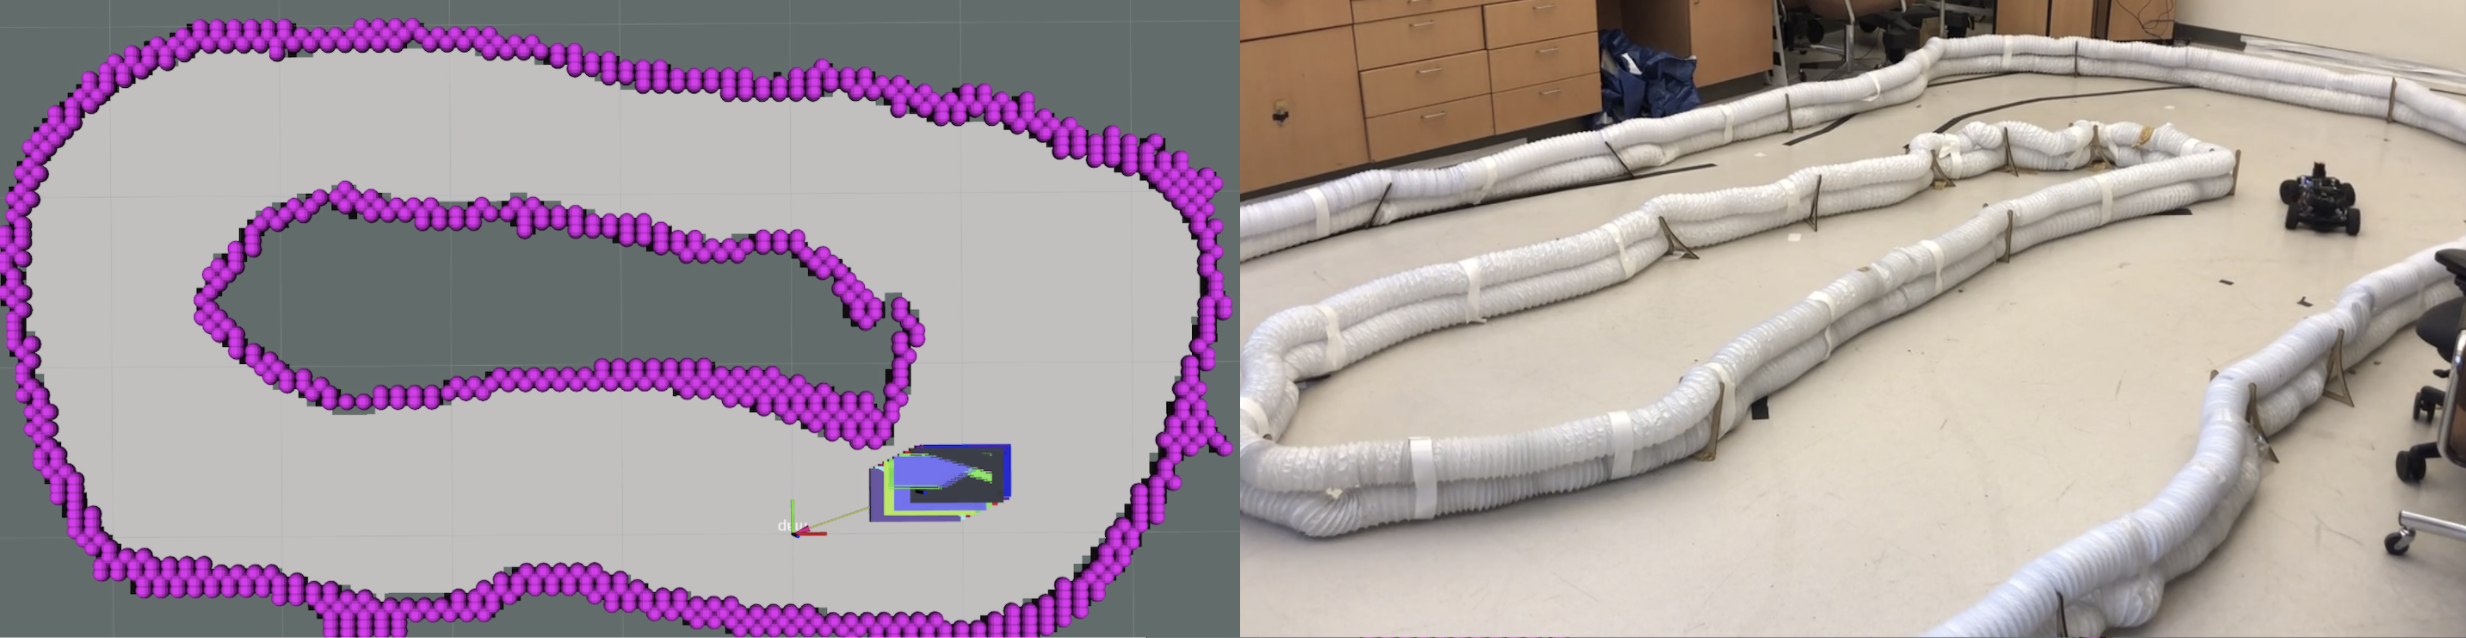
\includegraphics[width=\linewidth]{figures/sidebyside.png}
  \caption{Visualization of the hardware experiments on the F1/10 Platform, the magenta points are the point-discretization of the wall boundaries (not all points are visualized). Videos of the experiments can be found at}
%   \url{https://github.com/pmusau17/F1TenthHardware}.}
  \label{fig:lab_setup}
\end{figure}%
We ran 50 total experiments, 25 for each complex controller, on the hardware platform, where an experiment was defined as a completion of a single lap.\footnote{We sought to minimize any errors related to imperfect localization observations.} On average, the mean execution times for the hardware experiments were $11.3 ms$ and $10.6 ms$ for the end-to-end controller and reinforcement learning controller respectively. These results were significantly faster than the simulation experiments, but the simplex strategy was far more conservative. While the positive result of this observation was that there were no collisions in any of the experiments, the end-to-end controller was only used for $3.9\%$ of the time, and the reinforcement learning controller was utilized for a meager $5.3\%$ of the time. This is the primary reason that the mean execution time was much faster than the simulation experiments. 

Within the real-time reachability algorithm, the reachable-set computations terminate whenever an unsafe state is detected. The algorithm then restarts with half the step-size in order to refine the over-approximation error and determine if the ``unsafe'' declaration is spurious. This strategy continues, until the step size falls below a pre-specified threshold specified to guarantee numerical stability. On the hardware platform, this threshold was met consistently, which demonstrates the frequency of unsafe declarations. The subsequent testing in the simulation environment, where obstacles were removed thus reducing the uncertainty, provided evidence in support of this assertion. For further details on the termination conditions of the real-time reachability algorithm, see~\cite{Johnson2016}.







\section{Discussion}

Having evaluated the applicability of our approach and a timing analysis of the real-time reachability algorithm, we now present some observations based on our results in the light of the proverbial simulation to real-world gap that arises not only in the safety assurance research literature but also within artificial intelligence at large.

\subsection{Challenges Moving from Simulation to the Real World}

Moving from simulation to the real-world hardware platform saw a significant expansion in the frequency that the safety controller was used. This increased reliance on the safety controller is a direct result of \emph{sim2real} challenges in deep learning. Because the real world is inherently more noisy and more complex than the simulation environments that machine learning models are typically trained in, when these models are deployed in the real world, they are tasked with making generalizations on data that may significantly differ from their training distribution. Furthermore, this challenge is exacerbated by the reality of imperfect dynamic and sensor perception models\cite{ivanov2020case}.

The challenges that we faced during the transition from simulation to reality arose in two main fashions: the small track size and environment-induced sensor noise.

\subsubsection{The Small Track} The track shown in \ref{fig:racetrack} is much larger than the real world track we tested on, shown in \ref{fig:lab_setup}. At the narrowest point, the simulated track is $2m$ wide. In contrast, the widest part of our track is scarcely larger than that. The bulk of the racetrack has a width of less than one meter. Since $T_{runtime}$ is constant across the simulation and real world experiments, the real world vehicle spends the majority of its time forecasting unsafe actions due to its close proximity to the track walls. The hardware experiments were quite revelatory in motivating our desire to extend the current methodologies to integrate closed-loop reachability techniques. Our current assumptions are quite conservative. \diego{Why close loop? Mention that what these means is that at every control step (25ms) the input from the controller changes so it will mimic more closely the actual performance of the controller rather than the constant input assumptions}.

\subsubsection{Environment-Induced Noise} Noisy sensor data is expected because no sensor is always perfectly accurate. However, environment-induced noise refers to additional noise that exists because of differences in the environments. This is best highlighted in the case of the RL controller. The environment the agent trained in had smooth, solid walls. Meanwhile, our track is made out of a series of flexible vinyl duct piping hose segments\footnote{\url{https://www.amazon.com/dp/B01G198P8W?psc=1}}, which contain ridges and occasionally expose gaps in between the stacked structure. \diego{I don't like this last sentences in this paragraph. Technically, I assume that you could model the walls in the simulation to have this "wrinkles" if you use infinitely many "walls" in together with different shapes. We could technically create a track ourselves in that simulator and model the real-world track more realistically. We don't want to do this, but I don't like the "we cannot do this", they may come back with some arguments against this. I would use a different claim. By now I know that I sound very confusing, so feel free to jump in a zoom call if you want to discuss any of these comments} This introduces new input variations that cannot be replicated in simulation. Since the control is a ``black box'', we cannot know for sure how the policy will respond to these new inputs. Despite this challenge, we were able to get the vehicle to complete laps because of our simplex architecture. The overall performance might have been reduced, but we were able to ensure safe operation.

\section{Related Work}

As cyber-physical systems have become increasingly more complex in recent years, there has been a major thrust to develop techniques capable of assuring their safety at at runtime. % There has been a wealth of exciting works that attempt to prove the correctness of these systems prior to fielding them in their respective operational design domains, and a nice summary of these works is contained in the following papers \cite{Maler14,Tomlin2003,Doyen2018,Yang2017,Clark2013,Kwon2018}. In certain environments, however, complete or even partial verification may be infeasible due to the well-known state-explosion problem \cite{Valmari1998}, and the challenge may further be exacerbated by the opaqueness of the components considered. 
 This has led to the rise of \textit{simplex}, \textit{runtime assurance}, and \textit{runtime-verification} strategies, and it is within this context that we present our work.


\begin{table}[h]
\renewcommand{\arraystretch}{1.3}
\caption{Comparison of Online Reachability and Monitoring Methods %\ttj{if space is an issue, may want to use yes/no instead of true/false (or checkmark/xmark), and may want to make the header row multirow to make layout cleaner, or use an acronym for the header row titles and describe the acronym in this caption; I would add a row for this paper and highlight that in the earlier rtreach it has not been applied to LECs; also, are you sure any of these other approaches have real-time guarantees? are they just doing offline reachability, then monitoring online? may want to have a column for that or highlight that}
}
\label{tab:related_work}
\centering
\resizebox{0.7\linewidth}{!}{
\begin{tabular}{cccccc}
     & Real-Time & External & Evaluation & LEC & Online\\
     Tool Name & Guarantee & Libraries  & Platforms & Monitoring& Reachability\\
    \hline
 Rtreach-ML (this paper)& \checkmark & $\times$ & x86,ARM & \checkmark & \checkmark\\
 
 Rtreach \cite{Johnson2016} &  \checkmark & $\times$ & x86, ARM, AVR & $\times$ & \checkmark\\
 
 BACH2 \cite{Bu2011,BU2020} & $\times$ & \checkmark & x86     & $\times$ & \checkmark\\
 
 Flow* \cite{Lin2020}  & $\times$ & \checkmark & x86     & \checkmark & \checkmark \\
 
PHaVer \cite{Ti2014} & $\times$ & \checkmark & x86     & $\times$ & \checkmark \\
FaSTrack \cite{Bajcsy2019Provably} & $\times$ & \checkmark & x86    & $\times$ & $\times$ \\

 ARMTD \cite{holmes2020reachable} & $\times$ & \checkmark & x86  & $\times$ & $\times$ \\
 
  CORA \cite{Althoff2014} & $\times$ & \checkmark & x86  & $\times$ & $\times$ \\
  
  SafeTrafficWeaving \cite{LeungReach2020} & $\times$ & \checkmark & x86  & $\times$ & $\times$  \\
  
   ROSRV \cite{Huang2014} & $\times$ & \checkmark & x86  & $\times$ & $\times$ \\
   
    SOTER \cite{Desai2018,Desai2017} & $\times$ & \checkmark & x86  & $\times$ & $\times$ \\
    
    Modelplex/VeriPhy \cite{mitsch} & $\times$ & \checkmark & x86, ARM  & $\times$ & $\times$ \\
    % \vspace{0.1cm}
\end{tabular}}
% \footnotemark{CC refers to the complex controller, and SC refers to the safe controller.}
\end{table}%



The simplex architecture has been used widely in the research literature to provide guarantees for systems with unverified logic. The contexts in which it has been applied include aerospace systems \cite{SetoCaseStudy2000}, fleets of remote controlled cars \cite{Crenshaw2007}, industrial embedded infrastructure \cite{Bak2009Simplex,Yang2017}, and distributed mobile robotics applications \cite{Desai2018,Tran2020}. In \cite{Lin2020}, the authors utilize a reachability regime to guarantee the safety of an autonomous vehicle that makes use of a reinforcement learning controller for a way-point-following task. Most similar to this work in \cite{Tran2020}, the authors utilize a real-time reachability approach to verify that a group of quadcopters executing a distributed search mission defined by a series of waypoints is free from collisions. Their approach is implemented in simulation and can theoretically deal with over 64 quadcopters. These works primarily deal with developing provably correct motion planners, while the focus of this work is abstracting away the underlying nature of a set of ML components and reasoning about the consequence of their actions on overall system safety.



%In \cite{Desai2018}, Desai et al. propose an architecture for building reliable distributed mobile robotics by using a state-machine based language for safe event-driven programming. Like this work, their solution can be deployed within ROS, and the authors assume a known environment with static obstacles. However, their work is primarily focused on developing a provably correct motion planner, while this work projects the consequences of the control actions issued by a controller. In a similar work by Huang et al. \cite{Huang2014}, the authors present a run-time verification framework named ROSRV, which provides a specification language for ensuring safety and security properties within robotic applications. It allows for properties that can be expressed using temporal logic and regular expressions, and their techniques were demonstrated on a unmanned ground vehicle.

Closely related to simplex techniques are run-time assurance (RTA) methods and run-time verification (RV) methods. An intuitive explanation of these regimes can be summarized as follows. RTA techniques are tasked with ensuring the safe operation of systems with untrusted components, while run-time verification techniques monitor a system against presupposed formal properties at run-time 
%\cite{PETTERSSON200573,DesaiRV2017,Deshmukh2015,Masson2018,Akametalu2014,mitsch,Daws1998,Phan2020}. 
\cite{Masson2018,Akametalu2014,mitsch,Daws1998,Phan2020}. The distinction here is that while run-time assurance techniques may often utilize verification results, they may often also employ statistical techniques such as anomaly detection \cite{boursinos2020trusted} or simulation based strategies \cite{Clark2013}. %One such example is the work by Allen et al.\cite{Allen2014}, in which they utilize various machine learning techniques, mainly support vector machines and linear regression models, to approximate the solution to the real-time reachability problem. Their work is capable of being applied in low-resource, real-time environments but suffers from the downside that theoretical guarantees cannot be made using these techniques, only statistical ones. However, it demonstrated impressive results in improving state-of-the-art execution times by four orders of magnitude.

Finally, in recent years, researchers have begun to integrate traditionally non real-time approaches within real-time systems, making these approaches more amenable to real-time execution. These include viability kernel approaches that determine if a set of states remain within a predefined region \cite{Gurriet2018,Althoff2014}, as well as Hamilton-Jacobi (HJI) reachability techniques that deal with dynamical systems with general nonlinear dynamics and disturbances in uncertain environments \cite{Herbert2019,Bajcsy2019Provably,bansal2020hamiltonjacobi,Fisac2017,Chen2016,dhinakaran2017hybrid}. Specifically, \cite{Bajcsy2019Provably} and \cite{Althoff2014} were able to implement their techniques both in simulation and on hardware platforms. However, both papers used their respective real-time reachability results for safe real-time motion planning, while the work contained in this manuscript, primarily dealt with the construction and implementation of the simplex architecture. 

%In a similar vein, in \cite{LeungReach2020} Leung et al. proposed a safety-assurance control architecture based on HJI reachability for traffic weaving experiments. Their approach uses both forward and backward reachability techniques in order to integrate safety constraints into a model predictive controller tasked with trajectory generation. Their approach differs from this work in that they seek to minimize the intervention of safety control actions to situations where they are strictly required. 


Table \ref{tab:related_work} presents several state-of-the-art online reachability tools present within the literature, and summarizes their amenability to real-time operation. What distinguishes the methods presented in this work, is that they possess real-time guarantees and have been extended from \cite{Johnson2016} for the monitoring of machine learning models. Particularly, our work is to the best of our knowledge the only work that deals with perception controllers. We realize that there are numerous other interesting works present within this area, and to the best of our knowledge the aforementioned works are the most relevant to the methods presented within this manuscript.   

\section{Conclusions and Future Work}

In this work we proposed a simplex architecture for the safety assurance of a one-tenth scale autonomous car through the use of a real-time reachability algorithm compatible with the anytime computation model in the real-time scheduling literature. Our experiments conducted both in simulation and on an embedded hardware platform validate the real-time aspects of our approach and demonstrate its efficacy in assuring safety in different scenarios.

In the future, we hope to expand the work shown in this manuscript to include closed-loop reachability analysis. The current approach is limited to repeating the same control action for the duration of the reach time. This assumption results in an overly conservative use of the safety controller.%, which could prevent mission critical tasks from being performed in certain contexts. 
We did not consider closed-loop reach-set generation within our context due to the difficulties in developing an accurate sensor model. More specifically, it is not clear how to generate synthetic camera images that would provide a meaningful and useful reachable set. Even when the only sensor considered is the lidar, constructing an accurate sensor model is quite complicated, as shown by Ivanov et al. \cite{ivanov2020case}. In the future, we hope to work toward developing useful sensor models through the use of Generative Adversarial Networks, which are known for their ability to synthesize new examples that plausibly come from an existing distribution of samples \cite{Radford2016,Brock2018,goodfellow2014}.

\todo{Take a look at the references, some of them aren't displaying author's properly...}

\bibliographystyle{ACM-Reference-Format}
\bibliography{references.bib}


\appendix
%\section{Additional Experiments}
%\label{app:experiments}






\end{document}
\endinput